\documentclass[11pt,oneside]{memoir}
\usepackage[margin=0.5in]{geometry}

%\usepackage{showframe} % debug



\usepackage{titlesec}
\usepackage{verse}
\usepackage{tipa}
\usepackage{tabu}
\usepackage{xcolor}
\usepackage{multirow,bigdelim}
\usepackage{multicol}
\usepackage[generate,ps2eps]{abc}
\usepackage{mathptmx}
\usepackage{adjustbox}
\usepackage{textcomp}
\usepackage{pst-node}
\usepackage{tabularx}
\usepackage{rotating}
\usepackage{varwidth}

\usepackage{gensymb}
\usepackage{caption}

\newcommand{\sectionbreak}{\clearpage}
\newcommand\crule[3][black]{\textcolor{#1}{\rule{#2}{#3}}}
\newcommand\crekt[1][black]{\crule[#1]{3cm}{1cm}}
%\newcommand\crekt[1][black]{\fboxsep=10mm \fboxrule=1mm
%	\fcolorbox{black}{#1}{\null} }

\newcolumntype{Y}{>{\centering\arraybackslash}X}

\usepackage{graphicx}
\graphicspath{{./images/}}

\usepackage{fontspec}
%\fontspec{../font/flavangeometric.otf}
\newfontfamily\flavan[Path = ../font/, Scale=0.5]{flavangeometric}

\newcommand{\flav}[1]{  
	\begin{turn}{-90}
		\begin{varwidth}{10 cm}
			{\centering \flavan \hspace{-12pt} #1}
		\end{varwidth}
	\end{turn} }


\newcommand{\Flav}[1]{{\Large \flav{#1}}}

\newcommand{\ipa}[1]{/\textipa{#1}/}
\newcommand{\apa}[1]{[\textipa{#1}]}

\newcommand\setrow[1]{\gdef\rowmac{#1}#1\ignorespaces}
\newcommand\clearrow{\global\let\rowmac\relax}
\clearrow

\renewcommand{\abcwidth}{\dimexpr.7\linewidth\relax}

\title{Flavus}

\begin{document}

\maketitle

\chapter{The planet Flavus}

\section{Flavus}

Flavus is a smallish Earth-like planet orbiting a K0-class star. The common name refers to the planet's distinctly yellow tint, due to surface sulfur deposits.
%\section{Climate}

The axial tilt of Flavus is extremely modest, which leads to an imperceptible seasonal cycle and small polar circles. The temperature variation due to eccentricity of the orbit is even larger, though still minute. Therefore any given location on Flavus does not experience much difference in temperatures throughout the year.

The average surface temperature is significantly higher than on Earth. Only the polar regions, which host tropical-like climates, are inhabitable by humans. Intermediate latitudes are occupied by a vast, dry, acidic desert.

Flavus has currently very reduced tectonic activity and suffers from much more frequent asteroid impacts. The result is a relatively flat topography, mostly dominated by impact craters.

\section{The sulfur cycle}

Flavus slowly alternates between short periods of intense volcanism and long pauses of geological inactivity. During the former, copious amount of sulfur are produced, which are turned into fine dust and diluted into the sands of the planet.

When elemental sulfur concentration in sand exceeds a certain threshold, the possibility arises for a fire. Sulfur fires are awesome and terrifying, spreading quickly and then burning for days with a deep blue glow. Fires produce large columns of toxic sulfur dioxide.

The inverse direction is provided by the lifeforms native to the planet, the Plunts, which during photosynthesis consume sulfur dioxide in addition to carbon dioxide. Plunts store the absorbed sulfur in elemental form as small stones called *calculi*, which they release after their death.

At equilibrium, this feedback pair mantains a constant concentration of elemental sulfur in the sand and sulfur dioxide in the atmosphere. The latter (at ~ 10 ppm, to be compared with Earth's 1 ppm) is low enough for humans to survive, but still results in some permanently acidic rains and bodies of water.

\section{Flora}

The dominant native lifeforms of Flavus are a large class of plant-like creatures known colloquially as Plunts. Plunts perform a variant of photosynthesis in which sulfur dioxide can be also processed alongside carbon dioxide; the relevant combination of pygments (including clorophyll) gives almost all plunts a purple-blue colour.

Plunts however also possess animal-like traits; they are in fact often capable of limited locomotion and have primitive nervous-like systems. But it's the nature of their reproductive habits that is priceless for the human inhabitants of Flavus. The male organ of a Plunt consists of an elastic sac which is filled by sperm capsules over the course of a few months. When the pressure is sufficiently high, the sac bursts releasing the capsules, which are designed to be then transported by wind. The female organ instead produces an egg-like structure, a translucent white ovoid with a thick rubbery skin filled with a sugary protein syrup. The egg is topped by a receptacle, the true female organ. When a sperm capsule reaches a receptacle, a Plunt embryo is conceived and transferred to the egg.

The new individual is gestated for months inside the egg, which then hatches to reveal a cyan toadpole-like larva. The larva has some locomotive ability which it uses to get as far away as possible from the mother over the course of a few days. It then burrows the tail into the sand and becomes sessile, entering its adult stage.

Humans eat almost exclusively unfertilized plunt eggs, since they are relatively nutrient and not toxic like most of the organs of most plunt species. Growing eggs is relatively easy, consisting essentially in sealing the receptacle so that it cannot be fertilized. Plunt eggs are more agreeable when cooked, and are slightly alcaline with an ammonia-like smell.

Plunts do not have any signficantly rigid components. They are always elastic to some extent and their trunks are analogous to the tentacles of mollusks, being kept in position (or moved) through a hydraulic system. Their gummy purple skin is covered in a watery mucus, acting as an insulant to protect them from the extreme heat. 


\section{Fauna}

A branch of plunts have lost 

\chapter{Flavan civilization}

\section{Humans}

The most intelligent inhabitants on the planet are humans, or Flavans. What exactly they are doing there is unknown, and Flavans have no understanding of recollection of Earth, nor of the fact that they are not native to Flavus. Nevertheless, the planet is a harsh, inhospitable environment, with its dry, hot climate and acidic chemistry, and apparently Flavans have still not completely adapted accordingly, testifying that they haven't been around for more than a handful of millennia. Still, the small effect of these hardships on the bodies of humans are perceptible already. Flavans:
%{\flavan mn mng}
- grow 5 to 10 cm taller than Earthlings as a consequence of the lower gravity, which also increases chances of bone and heart-related diseases. 
- have very light skin, since UV radiation on the surface is low, owing to Flavus' star low temperature. A darker skin tone would facilitate vitamin D deficiency and has been quickly selected against.
- have respiratory and digestive systems slightly more suited for acidic environments. 

Flavans live in nuclear communities (*pak*), analogous to villages and averaging 200 individuals, based in oases in the arctic regions. Frequently, travelling groups will hop between oases by crossing the desert, carrying goods, knowledge, and money.

Two main ethnic branches inhabit the Arctic. The Demorog ("square-writing") occupy the pole, the upper, left, and lower regions, while the Bymarog ("flame-writing") live in a strip in the upper-right. It makes little sense to distuinguish smaller subdivisions as Flavan cultures, by virtue of their nature, constantly mix and rearrange.

\section{Fashion}

\section{Travel, shrooms and bannering}

Oases are small specks in a vast, unforgiving and extraordinarily bland desert, with very few recognizable points. A traveling group walking straight into the desert in a random direction could very well walk to their death without ever sighting a village. Orientation doesn't help much, as even a small error can build up and the destination could be missed entirely. How do travelers on Flavus manage to move around consistently? The solution is provided by the single largest living beings on the planet: shrooms.

Shrooms are gigantic mushroom shaped plunts, between 100 and 200 m tall, and inhabit primarily the polar desert, avoiding the excessive humidity of the oases. They have impressive root systems, sometimes even a kilometre across, to extract the necessary nutrients for survival. The "stalk" is relatively thin (two to three metres in diametre) but equipped with a powerful hydraulic pump is able to sustain the weight of the very large "cap", actually a disc-shaped layer of branches and leaf-organs. The cap itself is very light and little dense. Shroom (and their caps in particular) are home to rich ecosystems including parasites, symbionts, and predators.

Travelers use shrooms primarily as reliable reference points. Shrooms live easily for centuries, and skilled Masters can recognize individual shrooms from the shape of the cap, even from kilometres away. Shrooms are marked on maps and named, and traveling routes "hopping" from shroom to shroom are established. Not only: even if it wasn't for orientation, shrooms still make for attractive stops for travelers: the stalk can be cut to drip out sap, which is easily filtered for drinking, and its large (although distant, considering the Sun's low altitude) shadow, where the group can rest. Sadly, they cannot literally stop in the cap's shadow and drop the tents: the shroom is so tall that the shadow moves too fast throughout the day, forcing travelers to continuously move every half-hour.

Upon passing by an undiscovered shroom, the Master will mark it with a banner of their village (or occasionally one of the recently visited villages), a flag-like piece of cloth bearing the pak name. These banner are manufactured in advance by children in the pak and travelers always carry a few. The banner has a pouch in which travelers insert "update documents": writings reporting on their travel, maps, news on the recently visited villages, general updates, and a bit of gratuitous personal diary. The next visitors to the shrooms can then enjoy this information and add their own to the shroom's archive. Travelers communicate much more information through bannering than through actually meeting in travel, which happens rarely.

A shroom banner for the Ramy village, with embroidery in geometric style. Below the word *ramy* itself, the map symbol for a village is used as a shorthand for pak. On the bottom, a pouch for update documents.

\section{Villages}

\section{Sex, Gender and Parenthood}

Flavans don't like children. Even in what is relatively speaking an oasis, the harsh lifestyle makes survival of the community the first preoccupation; procreation, and thus a noticeable population increase in a small village is seen as damaging. Bearing child is therefore heavily regulated and the mother is required to pay the *pak* authority a fee whose value is regularly updated depending on the village's situation. Failure to produce the money can result in expulsion.

This "demographic phobia" has its origin in Flavan folklore of villages destroyed by overpopulation, and results in very unusual ideas on sex drive, reproduction, gender, and the role of children in society. Children are perceived as "impure", "indecent" or more precisely "unstructured"; physician Baryk-t Ardeman describes the process of growing a child into an adult as akin to the drying of gum-birch skin, removing its toxic "blue" essence to reveal a structured individual:

*the child is born as an amalgalm of the elements, imbibued with blue as the skin of the gum-birch. Living amongst the yellow, it is dried, and the blue drips, and it takes face.*

The genitals and nose of children are always to be covered in public, and the distinction between child and adult is stronger than even that between male and female, a feature reflected in the Flavan language. A child is grown and educated by his mother only; there is no concept of fatherhood on Flavus. The biological father has no responsibilities nor rights concerning the child. The closest idea to fatherhood is a form of tutorage in which an adult (almost always male) trains a child in various skills, most importantly reading and writing and the basic of travelling; it's not uncommon for an emotional bond to develop, nor is it frowned upon. A child can have any number of tutors.

Children become adults as they reach ... Visits (... Earth years) of age, at which point they are "uncovered" in a ceremony. To emphasize that the adult Flavan is not far from being considered a distinct person from themselves as a child, adults count their age starting from their uncovering.

Because reproduction is almost always seen in such a negative light, Flavans rationalize the sex drive as "intrinsic suffering" to being alive, and in alignment with their philosophy believe that like all forms of pain it should be embraced and redirected towards good or constructive purposes. Therefore, they understand the need for recreational sex. There is variety in the sexual habits of Flavans, but an obvious constraint is that vaginal penetration is forbidden (unless the woman is prepared to have - and pay for - a child). Demorog do not really perceive any difference between male and female and tend to engage in often short, vaguely monogamous relationships, either heterosexual or homosexual. Bymarog forbid all recreational heterosexual contact, but gladly accept homosexual (male and female) pairings, but do not have any concept of relationship or commitment at all.

The body of a Flavan is considered their most prized possession, because of the suffering associated with owning it. (In fact, the female body is regarded as even more valuable, because of the menstrual cycle and the associated physical pain and discomfort). Therefore, Flavans classify rape as a form of theft, which is an unforgivable sin. All forms of rape are punished with expulsion, in addition to the child fee in case the rape results in a pregnancy.

The reason for reduced gender differences in Flavan society is mostly that there is neither much hunting, nor child-bearing to do on Flavus. (Side note: Flavans would not be able to understand an arrow symbol). Gathering, building and travelling require skills common to both sexes and almost all roles in Flavan society include men and women in comparable fractions. Flavan grammar does not distinguish male and female, and while most proper names are indeed gendered, a good portion of them are Unisex. In fact, the very physician quoted above, Ardeman of the Baryk village, bears such a name and it's not possible from their writing to infer whether they were a man or a woman.

\section{Culture}

When they laugh, Flavans take out their tongue and keep it between their teeth.

\section{ Science}

\section{Astronomy and Religion}

In addition to the fixed stars, the only two astronomical objects that the Flavans are aware of are the Star and the Wanderer (Vulcan being too close to the Star to be visible). Flavans believe these two objects to be identified with two gods, 

The Wanderer is a bright, spectacular sight when in opposition, that is when it is closest to Flavus, and reaches maximum altitude at midnight. In fact, Flavans measure years as spanning between consecutive oppositions (which they call "visits") of the Wanderer, instead of through the motion of their sun on the fixed stars as it is done on Earth. Thus, Flavans prefer the synodic period of the Wanderer with respect to Flavus, rather than Flavus' own sidereal period, to act as a measure of time. This choice is coherent both with the absence of detectable seasons and with the secondary role the "fixed" stars have in Flavan cosmology.

\section{Food}

\section{Magic and Medicine}
 

\newpage
\section{Writing}

Flavan writing arises from the practical need of mapmaking. Since mutual intelligibility is key, Flavans essentially all use one unified script, but with distinct styles of rendering shapes. The Flavan script was originally an alphabet (with consonant and vowels being represented by distinct glyphs) but has transitioned into an abugida as consonant and vowel glyphs have fused into new forms. It is written vertically, more precisely top-to-bottom, right-to-left; words within a single column are separated by a dot.

The most bizzarre aspect is the writing tool Flavans use, the pen-leech. Pen-leeches are parasitic worm-like animals distributed throughout the Polar regions, and which feed on large plunts, in particular shrooms. The pen-leech attaches to the trunk of the plunt through its two cartilage fangs; when secured to the skin it squeezes out a corrosive mucus, essentially digesting the host externally, then sucks back the mucus into its body for absorption. This cycle is repeated. Pen-leeches are barely taxing on the gigantic shrooms and the latter can often host hundreds or thousand of parasites with no real damage to itself. Flavans exploit the leeches' sucking and splurting ability to use them as pens. Travellers collect a few as they hop by a shroom. Once brought home to the village, they are prepared as such:

\begin{itemize}
\item The brain node, in the posterior of the creature, is cut off alongside the vestigial root. This kills the leech :(
\item The carthilage fangs are removed carefully to retain a smooth, circular mouth.
\item The leech is cleaned and hanged to dry out the sap
\end{itemize}

The pen-leech, now more rigid and elastic, is then ready to be used similarly to a fountain pen, sucking in an ink produced from ashes, and releasing it on paper when squeezed. This gives rise to the characteristic roundish strokes in Flavan writing. Pen leeches do not last more than a month before starting to rot, and thus must be replaced frequently - therefore, there is no such thing as a "luxury" pen-leech, even though a skilled pen-leech preparer is highly regarded.

Writing styles can be split roughly into three general categories:

\begin{itemize}
\item The Demorog "geometric" style, mostly employed in embroidered or chiseled designs or in very large writings (such as on walls). Occasionally also used in tattoos and maps.
\item The Demorog "cursive" style, for maps, letters, books, and everything in pen-leech.
\item The Bymarog "flame" style
\end{itemize}

Here are the words *Demorog* (right) and *Bymarog* (left) themselves, written respectively in geometric, cursive, and flame style.

The words denoting the two ethnic groups themselves (Demorog = square-writing, Bymarog = flame-writing) refer to the appearance of these writing styles.

A few designs for the word *moshl* ("mother")

\section{Colours}

Green-Grey

Pink-Red-Yellow

Blue-Purple



\begin{tabu}{c l c}

	\crekt[white]	& \rdelim]{1}{3mm}[White] &\\
\crekt[yellow] &  \rdelim]{3}{3mm}[``Yellow''] &\\
\crekt[orange] & &\\
\crekt[red]	& &\\
\crekt[magenta]	& \rdelim]{4}{3mm}[``Blue''] &\\
\crekt[purple] & &\\
\crekt[blue] & & \\
\crekt[cyan] & & \\
\crekt[green] &  \rdelim]{2}{3mm}[``Green''] &\\
\crekt[gray] & & \\
\crekt[black] &  \rdelim]{1}{3mm}[``Black''] & \\

\end{tabu}

\section{Music}

Flavan music is strongly percussive and often based on a specific 5/4 rhythm:

\begin{abc}[name=rhythm]
X: 1 % start of header
K: C % scale: C major
M: 5/4
c3 c3 c2c2  |
\end{abc}

%\begin{abc}
%X:4
%T:Cronin’s Hornpipe
%R:hornpipe
%S:Keenan and Glackin
%E:7
%M:C|
%L:1/8
%K:G
%BA|GABc dBde|gage dega|bage dBGB|cABG A2BA|!
%GABc dBde|gage dega|bage dBAB|G2G2 G2:|!
%fg|afd^c d2ga|bged e2ga|(3bag  (3agf gedB|(3cBA AG AcBA|!
%GABc dBde|~g3e dega|bage dBAB|G2G2 G2:|!
%\end{abc}
%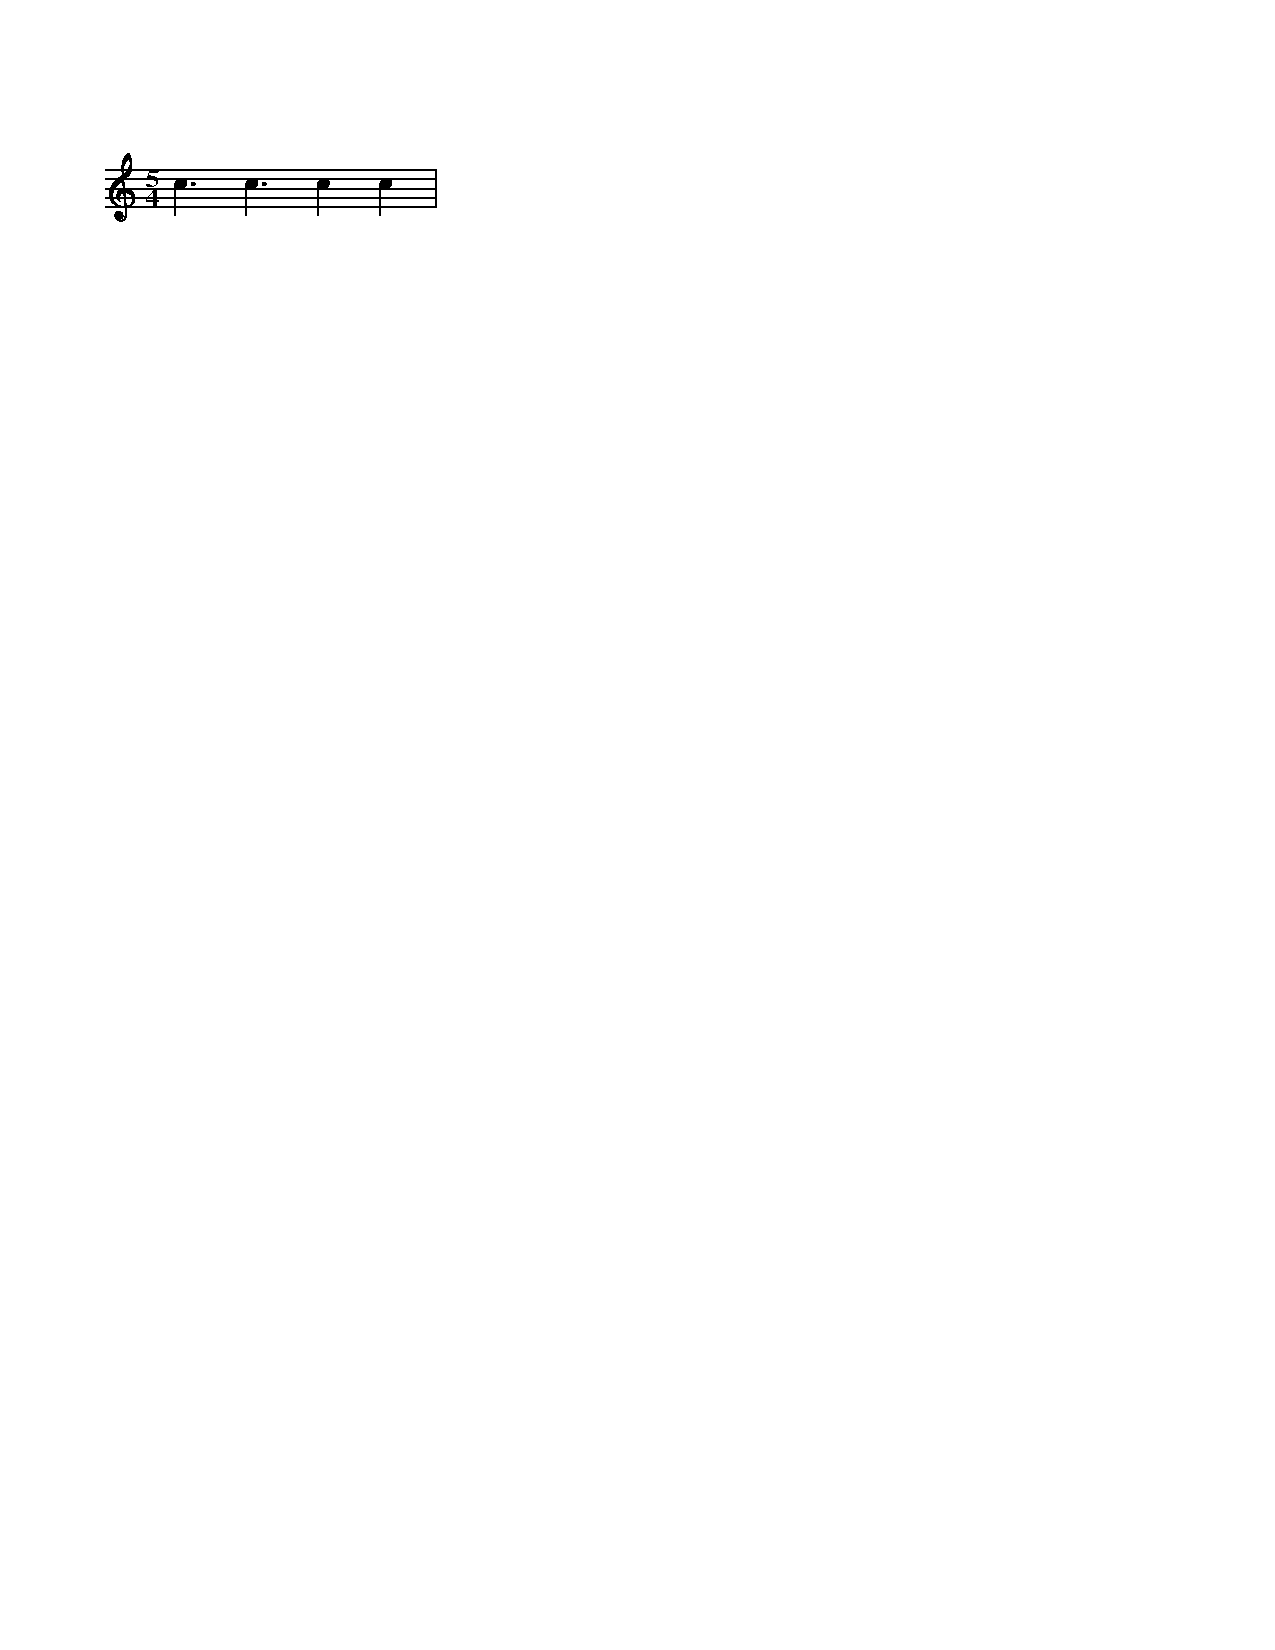
\includegraphics{rhythm}

And melodies are played in a hexatonic scale:

\begin{abc}[name=scale]
X: 1 % start of header
K: G 
L: 1/4
M: 5/4
CDEFGA|c
\end{abc}

%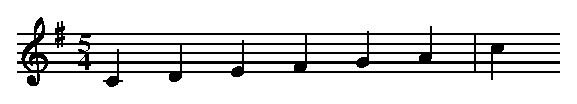
\includegraphics{scale}

(This representation in terms of equal temperament notes is of course an approximation). This scale can be seen as an extension of the major pentatonic to include the maximally dissonant flat fifth / sharp fourth, or equivalently as a subset of the western lydian scale. The inclusion of the tritone interval, a modern and daring device which on Earth had essentially never been truly appreciated as anything else than \emph{diabolic} before Romanticism, is baffling - the other intervals are instead extremely natural and based on small integer ratios. (Arguably, the pentatonic scale is likely universal to all humans). 

Music is played by traveling "bands" composed of a Drummer, a Lead vocalist, and one or two Backing vocalists. Songs take a vaguely choral form as the backing vocalist open by singing the title/refrain in a constant note; this works as an "introduction" to the piece of music, and also establishes the fundamental note and the tempo. The Drummer joins in and the Backing continues to hum the refrain on the fundamental. After, the Lead introduces the main melody and lyrics, harmonizing on the backing's drone. Flavan music is thus essentially biphonic, though the bass is simply a drone, very rarely changing. Lyrics almost always tell a story, either humorous (and vulgar) or tragic, and the refrain itself is very often an ironic twist on the subject that is only understood after the main lyrics are presented, even though it gets continuously repeated throughout the song. Sometimes, the refrain even rhymes with the last verse of the lyrics.

A translated Demorog example:


\poemtitle{It's empty like death}

\begin{verse}
\emph{(backing starts droning: ``it's empty like death'')}

Abar of the Shefe village has\\
brimstone hair and silver sweatdrops\\
Rkon of the Bybang village wants\\
the sweet green breasts\\
that Abar of the Shefe village has.

\end{verse}

\begin{verse}

But everytime that Rkon comes\\
to Shefe village and Abar's tent\\
Abar's mother is always there.

\end{verse}

\begin{verse}



Abar writes a letter then,\\
come to visit in seven days,\\
and no one will be in the tent.\\
\end{verse}

\begin{verse}


Rkon of the Bybang village reads,\\
Rkon walks from here to there\\
sulfur feet he has to have\\
He enters Abar's tent and


\emph{(it's empty like death)}

\end{verse}

In this interesting example, the refrain is doubly deceiving as it also sets up a dramatic mood which is then inverted by the humorous subject. The expression "empty like death" refers to the fact that the internal organs of dead plunts decay much faster than their skin, which leaves them with a "deflated balloon" appearance. The curious combination "green breasts" makes sense in the context of Flavan perception of colour, and probably refers to a grayish-pinkish hue of very pale skin.





\section{Psychedelics}

\chapter{The Flavan Language}


\pagebreak
\section{Phonology and phonotactics}

The phonetic inventory of Flavan is most conveniently presented by means of their own organization in terms of an ``alphabet'', which is a list of allowable consonant clusters and single vowels. Curiosly, they arbitrarily separate consonantal sounds into ``common'' and ``uncommon'', crudely reflecting the frequency of those phonemes in spoken language. The following chart lists the Flavan names for the phonemes, their average Demorog and Bymarog pronunciations, their romanization, and also introduces the corresponding glyphs in the Flavan abugida, which will be introduced later.

%\begin{multicols}{2}

\begin{adjustbox}{center}
{\large
\begin{tabu}{c c c c c }
	\multicolumn{5}{c}{The ``Males'' (common consonant clusters)}\\
	\rowfont{\small}
	Glyph & Rom. & \multicolumn{2}{c}{Pron. (Dem./Bym.)} & Name \\
	\hline 
\flav{-}	& None	& //\footnotemark		& \apa{}		& pode\\
	\flav{m}	& m	& \ipa{m}	& \apa{m}	& ma \\ 
	\flav{p}	& p	& /p/		& \apa{p}		& pa\\
	\flav{b}	& b	& /b/		& \apa{b}		& ba \\
	\flav{n}	& n	& \ipa{n}	& \apa{n}	& na \\ 
	\flav{t}	& t	& /t/		& \apa{t}		& ta\\
	\flav{d}	& d	& /d/		& \apa{d}		& da\\
	\flav{ng}	& ng	& \ipa{N}	& \apa{N}	& nga \\ 
	\flav{tt}	& tt	& \ipa{t:}	& \apa{t:}	& kotta\\
	\flav{dd}	& dd	& \ipa{d:}	& \apa{d:}	& kodda\\
	\flav{shl}	& shl	& /\textesh l/	& [\c{c}l]	& shla\\
	\flav{k}	& k	& \ipa{k}	& \apa{P}	& ka\\
	\flav{g}	& g	& \ipa{g}	& \apa{g}	& garyn\\
	\flav{dh}	& dh	& \ipa{D}	& \apa{z}	& dhe \\
	\flav{dhl}	& dhl	& \ipa{Dl}	& \apa{zl}	& dhla \\
	\flav{s}	& s	& \ipa{s}	& \apa{s}	& syk \\
	\flav{sh}	& sh	& \ipa{S}	& \apa{\c{c}}	& shyk \\
	\flav{f}	& f	& \ipa{f} (or \apa{v}) & \apa{v} & fa\\
\flav{r}	& r	& \ipa{r}	& \apa{l} & ra \\
\flav{rd}	& rd	& \ipa{rd}	& \apa{rd}	&rda \\
\flav{rk}	& rk	& \ipa{rk}	& \apa{rk}	&rka \\
\flav{rb}	& rb	& \ipa{rb}	& \apa{rb}	&rba \\
\end{tabu}
\begin{tabu}{c c c c c}

	\multicolumn{5}{c}{The ``Females'' (rare consonant clusters)}\\
	\rowfont{\small}
	Glyph & Rom. & \multicolumn{2}{c}{Pron. (Dem./Bym.)} & Name \\
	\hline 
	\flav{bl}	& bl	& \ipa{bl}	& \apa{bl}	& bla \\
\flav{ttf}	& ttf	& \ipa{t:f}	& \apa{t:f}	& kottfa \\
\flav{ttl}	& ttl	& \ipa{t:l}	& \apa{t:l}	& kottla \\
\flav{ttk}	& ttk	& \ipa{t:k}	& \apa{t:P}	& kottka \\
\flav{ttg}	& ttg	& \ipa{t:g}	& \apa{t:g}	& kottga \\
\flav{rg}	& rg	& \ipa{rg}	& \apa{rg}	& rga \\
\flav{sg}	& sg	& \ipa{zg} (or \apa{Dg})	& \apa{zg}	& zga \\
\flav{gm}	& gm	& \ipa{gm}	& \apa{gm}	& agme \\
\flav{rm}	& rm	& \ipa{rm}	& \apa{lm}	& rma \\
\flav{pd}	& pd	& \ipa{pd}	& \apa{pd}	& pda \\
        	
		\hline\hline
		\multicolumn{5}{c}{The ``Children'': Vowels}\\
		\rowfont{\small}
		Glyph & Rom. & \multicolumn{2}{c}{Pron. (Dem./Bym.)} & Name \\
		\hline 
None		& a	& \ipa{a}	& \apa{a}	& atta\\
\flav{e}	& e	& \ipa{e}	& \apa{e}	& etta\\
\flav{y}	& y	& \ipa{1} (or \apa{ju})	& \apa{u} (or \apa{ui}) & ytta \\
\flav{o}	& o	& \ipa{o} 	& \apa{o} & ordar\\




\end{tabu}
}
%\end{multicols}
\end{adjustbox}

\footnotetext{The \textbf{pode} (//) is not an actual phoneme, but simply a vowel carrier necessary to represent a vowel without a preceding cluster in the Flavan script.}


A flavan word is just an alternating sequence of consonant clusters and vowels (with at least one vowel). So, if C is a cluster and V is a vowel, words can be V, CV, VC, CVC, VCV, CVCV, \emph{etc}. Any clusters can be at the beginning, middle or end of a word.

It is occasionally possible for two vowels to be consecutive (VV) as a consequence of affixing. In that case, if the vowels are different they form a diphthong.

\subsection{Pronunciation rules}

\begin{itemize}
	\item \ipa{1r} becomes the syllabic consonant \apa{\s{\*{r}}}. Example: \textbf{yrk} \flav{yrk} \ipa{\s{\*{r}}k}, \emph{and}
	\item \ipa{e} and \ipa{o} when stressed open up to \apa{E} and \apa{O} respectively. Example: \textbf{borag} \flav{borag} \ipa{"bO.rag}, \emph{sulfur}
	\item word-final \ipa{l} after a consonant becomes syllabic \apa{\s{l}} (this creates a new syllable). Example: \textbf{moshl} \flav{moshl} \ipa{"mO.S\s{l}}, \emph{mother}
	\item a vowel following \ipa{N} will become nasalized. Example: \textbf{ngon} \flav{ngon} \ipa{N\~on}, \emph{I (ergative)}
	\item word-final \ipa{D} becomes geminated: \apa{D:}. Example: \textbf{my agaredh} \flav{my\\agaredh} \ipa{m1aga'reD:} \emph{goodbye}
\end{itemize}

\subsubsection{The tell-tale \emph{ytta}}

The phoneme \ipa{1} represented by the letter \textbf{ytta} (\textbf{y}) requires clarification. We have already considered the merge \ipa{1r} \textrightarrow\apa{\s{r}}, so we exclude this case here. It should be noted that \apa{1} is an average sound over all dialects, and that the essential characteristic that sets it apart from \ipa{e} and \ipa{o} is only its being closed. Therefore all closed vowels, rounded and unrounded, and closed\textrightarrow closed dipththongs are allophones for \ipa{1}. Different dialects and accents of Flavan however employ different subsets of allophones with different pronunciation schemes. This allows a Flavan speaker to identify the origin of a speaker from his pronunciation of \textbf{ytta}s and his choice of closed vowels, a phenomenon known as the \textbf{tell-tale ytta} (\textbf{ytta robordam}).

The ``standard'' pronunciation (Central Demorog) has only \emph{unrounded} vowels accompained by approximants, and no diphthongs. The idea is that the three different positions of unrounded back vowels (\ipa{i 1 W}) are employed when the ytta is between consonants of similar place of articulation, and a ``slide'' from one to another is made if the consonants are differently articulated. More simply: the consonant before is the row and the one after the column, the depicted sound is that of \textbf{y} when sandwiched between them.

\begin{center}
\begin{tabular}{c|c|c|c}
        & \ipa{mpbtfnlt}  & \ipa{kg} & \ipa{N}\\
        \hline\hline
        \ipa{mpbtfnlt} & \apa{i} & \apa{j1} &  \apa{jW}    \\ \hline
        \ipa{kg} & \apa{1j} & \apa{1} & \apa{jW} \\ \hline
        \ipa{N} & \apa{\textturnmrleg i} & \apa{W} & \apa{W}
\end{tabular}
\end{center}

If either side doesn't have consonants the values on the diagonal are taken.

Another interesting system is that of the Bymarog. They do have more in the rounding department, but no approximants: 

\begin{center}
\begin{tabular}{c|c|c|c}
        & \ipa{mpbtfnlt}  & \ipa{kg} & \ipa{N}\\
        \hline\hline
        \ipa{mpbtfnlt} & \apa{i} & \apa{u} &  \apa{u}    \\ \hline
        \ipa{kg} & \apa{y} & \apa{1} & \apa{u} \\ \hline
        \ipa{N} & \apa{y} & \apa{u} & \apa{u}
\end{tabular}
\end{center}

\section{Stress and intonation}

Absolute vowel lengths are not distinguished phonemically in Flavan; however there is a notion of the longest and loudest (\textbf{stressed}) syllable in a word as compared with all the others (\textbf{unstressed}). Stress, or accent, in each word is applied according to precise rules, thus it cannot help distinguishing single words lexically; however it helps in communicating word boundaries, which can often help disambuguating. Stress is (very optionally) marked with a grave accent: \`a \`e \`o \`y in romanization (an accented l is not necessary since it is impossible for \apa{\s{l}} to be stressed). The rules for stressing a word with at least two syllables are as follows, to be applied in order:

\begin{enumerate}
	\item Stress is placed on penultimate syllable\footnote{the syllabic liquids are counted here. So \textbf{mashl} has two syllables, with nuclei \textbf{a} and \textbf{l}.}.
	\item If last syllable's nucleus is \textbf{a}, stress moves to the last syllable.
	\item If there is gemination in the cluster between penultimate and last syllable nucleus, stress moves to penultimate syllable.
	\item If the word ends in a cluster with gemination, stress moves to last syllable.
\end{enumerate}

An example: \textbf{kottla} \flav{\hspace{-5pt}kottlaa} (the cardinal numeral 4096) starts as \textbf{kòttla} according to rule 1. Rule 2 changes to \textbf{kottlà}, but rule 3 changes back to \textbf{kòttla} because of the geminated t. Rule 4 does not apply, as there is no final cluster. Thus \textbf{kòttla} is the final stress, and pronunciation is \ipa{"kOt:la}.


\section{Word order and morphosyntactic alignment}\label{alignment}

Flavan could be briefly described as a SOV language, meaning sentences follow the order subject-object-verb. For example, \emph{Shlem eats a dhlorg} could be translated as

\begin{center}
	\textbf{Shlem dhlarg rbam}\\
	Shlem.SUBJECT dhlorg.OBJECT eats\\
	\Flav{shlem dhlarg rbam}
\end{center}

However, this is not strictly correct and potentially confusing because Flavan has ergative-absolutive alignment. This means that the distinction between subject and object is not well-defined, while entities involved in an actions are instead classified as \textbf{agents} (subjects of transitive actions) or \textbf{patients} (objects of transitive actions or subjects of intransitive actions). In fact, Flavan is unusual in being more ``thorough'' in its ergativity than most earthly ergative languages. The word order is thus better described as agent-patient-verb, or APV. 

The nouns/pronouns that represent the agent/patient are declensed respectively in the \textbf{ergative}/\textbf{absolutive} cases. This means for example:

\begin{center}
	\textbf{ngon nar rbap} - \emph{I ate it}\\
	me.ERG it.ABS ate\\
	\Flav{ngon nar rbap}\\
	\vspace{10pt}
	\textbf{ngan bodark} - \emph{I slept}\\
	me.ABS slept\\
	\Flav{ngan bodark}
\end{center}

The sleeper (actor of an intransitive action) is treated like the eaten (object of a transitive action).

There is yet another alien element to Flavan syntax, the \textbf{wanter}. This can only appear if the verb is in the deontic mood (which expresses wishes, hopes or orders) and specifies who actually desires the action to happen. The wanter is declensed in the \textbf{dative} case, and comes after the verb. Example:

\begin{center}
	\textbf{Shlem dhlarg rbem ngof} - \emph{I want Shlem to eat the dhlorg} \\
	Shlem.ERG dhlorg.ABS eat.DEONTIC me.DAT\\
	\Flav{shlem dhlarg\\ rbem ngof}
\end{center}

Thus to conclude, the order could be simplified as APVW, or

\begin{center}
	Agent - Patient - Verb - Wanter
\end{center}

Note that while the order is very strict, all elements are actually mandatory, except for the verb.

\subsection{No antipassive voice}

Flavan ``does not have the antipassive'', which means transitive verbs without an object are \emph{still} treated as transitive. So \emph{I ate} is still \textbf{ngon rbap}, with ``me'' in the ergative case, while a language with antipassive voice might shift to the absolutive.

\subsection{The \textbf{ak} \emph{copula}}

The verb \textbf{ak}, meaning \emph{to be} in the sense of copula (i.e. ``the sky is blue'') has two unusual properties that deserve care:

\begin{itemize}
	\item It is \textbf{transitive}. The complement to the subject is literally treated as an object and thus takes the absolutive, while the subject itself is in the ergative. Example:
\begin{center}
	\textbf{Shlem katarotta attk} - \emph{Shlem was a woman}\\
	Shlem.ERG woman.ABS was\\
	\Flav{shlem katarotta attk}
\end{center}
	\item It always disappear in the present indicative, an example of \textbf{zero copula}. So \emph{Shlem is a woman} is literally \textbf{Shlem katarotta}. It readily reappears when conjugating the verb in any way, for example in the interrogative mood: \textbf{Shlem katarotta yk?} - \emph{is Shlem a woman?}. Thus, the specific word \textbf{ak} does not actually exist in Flavan.
\end{itemize}

\pagebreak

\section{Nouns}

Nouns are declensed according to number and case.



\subsection{Number}

Three main numbers are always present: \textbf{singular}, \textbf{dual} and \textbf{plural}. 

\subsection{Case}

\subsubsection{Ergative}

The ergative case's role was already explained in section \ref{alignment}.

The ergative case is \emph{unmarked} and it's the default (``lemma'') form for nouns.

\subsubsection{Absolutive}

The absolutive case's role was already explained in section \ref{alignment}.

The absolutive is marked by \textbf{first vowel opening} (FVO), the shift in the \emph{first} vowel of the noun as:

\begin{tabular}{c | c c c c}
	Ergative first vowel & a  &e  &o & y\\
	Absolutive first vowel & a & a & a & o
\end{tabular}

and in addition, the number suffix becomes a number \emph{pre}fix.

\subsubsection{Genitive}

The genitive signifies possession (alienable or inalienable), and origin.

It is marked by the suffix \textbf{-t}. A few irregular genitives arise for some noun endings:

\begin{tabular}{c | c}
Ergative & Genitive\\
-g	& -kt\\
-t	&  -tt
\end{tabular}

If a noun is not part of these exceptions, and the suffix \textbf{-t} were still to create a nonexisting cluster, \textbf{-et} is used instead.

\subsubsection{Dative / Locative}

The dative marks the receiving end of giving or communication. The locative instead signifies the noun represent a place where the action happens or towards which motion is intended.

The dative is built through the prefix \textbf{o-}.

\subsubsection{Ablative / Instrumental}




\pagebreak

\section{Adjectives}

Adjectives are incredibly simple in Flavan: they are not declensed nor do they align with the nouns they complement. Because of this adjective position is crucial for clarity; adjectives always come right after the noun they refer to.

\subsection{Intensity}

The strength of adjectives can be modulated by a series of constructions.

\begin{itemize}
	\item \textbf{strengthening} (e.g. \emph{very}) is realized through \textbf{first syllable reduplication}. For example, \textbf{ttla} \emph{good-looking, beautiful} becomes \textbf{ttlyttla}, \emph{very beautiful}.
	\item \textbf{inversion} (not to be confused with negation) turns an adjective into its opposite, and it's marked by the prefix \textbf{dhla-}. Example: \textbf{dhlattla} \emph{ugly}.
\end{itemize}

\subsection{Comparison}

Comparison is subtle and alien in Flavan. It is expressed by means of \emph{comparison verbs}, most importantly \textbf{merak} and \textbf{dhlamerak}, very vaguely translatable as \emph{``to be more this than''} and \emph{``to be less this than''}. To express that X is more A than Y, one says that X \textbf{meraks} A \emph{to} Y, or said otherwise the object of comparison takes the dative case. For a concrete example:

\begin{center}
	\textbf{Shlem ttla o-Rkon merak} - \emph{Shlem is more beautiful than Rkon}\\
	Shlem.ERG beautiful Rkon.DAT merak.IND.PR\\
	\Flav{shlem ttlaa\\orkon merak}
\end{center}

This verbal form of comparison is preferrable, but if strictly necessary a true comparative adjective can be formed through the agent participle of the comparison verb (see section \ref{verbs}).

The possible comparison verbs are

\begin{tabular}{c | c}
	merak & more than\\
	dhlamerak & less than\\
	kobymat & equally as\\
	dhlakobymat & differently from
\end{tabular}

%Superlatives can be formed by replacing the dative with the expression \textbf{obydhek}, roughly ``\emph{than all}''.

\pagebreak


\section{Verbs}\label{verbs}


\begin{center}
	\ipa{deN\~o"nak}, \emph{glistening, shimmering}
\end{center}

\begin{center}
	{\Huge \rnode{prefix}{\psframebox{de}}\rnode{stem}{\psframebox{ngon}}\rnode{vowel}{a}\rnode{coda}{\psframebox{k}}}
\end{center}

\bgroup
\def\arraystretch{1.5}

\begin{tabularx}{\textwidth}{>{\rowmac}X|>{\rowmac}X|>{\rowmac}X|>{\rowmac}X<{\clearrow}}
	\setrow{\bfseries} \rnode{prefixexp}{Prefix modifiers} & \rnode{stemexp}{Stem} & \rnode{vowelexp}{Mood Vowel} & \rnode{codaexp}{Tense Ending} \\
	mark participles, inversion, etc.	& carries root meaning alongside ending & carries mood & carries relative tense\\
	e.g. \emph{de}: marks patient participle & e.g. \emph{ngon\_k}: (int.) to shine, to glisten & e.g. \emph{a}: indicative mood & e.g. \emph{-k}: relative present
\end{tabularx}

\egroup

\ncdiag[arm=2mm,angleA=-90,angleB=90]{->}{stem}{stemexp}
\ncdiag[arm=2mm,angleA=-90,angleB=90]{->}{prefix}{prefixexp}
\ncdiag[arm=2mm,angleA=-90,angleB=90]{->}{vowel}{vowelexp}
\ncdiag[arm=2mm,angleA=-90,angleB=90]{->}{coda}{codaexp}


\setlength{\columnseprule}{0.4pt}
\setlength{\columnsep}{1.5 cm}

\begin{multicols}{2}
	\subsection{Tense}
	Conjugated tense is relative to the absolute tense of the proposition, which is instead established through specific time adverbs or inferred from context (e.g. inherited from the previous sentence). So the three conjugated tenses, \textbf{present}, \textbf{anterior}, \textbf{posterior} mean the action is performed respectively simultaneously, before, or after the current absolute time.

	Relative tense is marked by the final consonant cluster; verbs are arranged in classes according to their present tense ending, with the -k class the most populated.

	\vspace{10pt}

	\begin{tabularx}{\columnwidth}{>{\rowmac}Y>{\rowmac}Y>{\rowmac}Y<{\clearrow}}
		\setrow{\bfseries}Present & Anterior &Posterior \\
		\hline
		-k & -ttk & -dh \\
		-rd & -rk & -r \\
		-t & -tt & -d \\
		-tt & -ttk & -dd \\
		-rg & -rk & -ng \\
		-m & -p & -ng
	\end{tabularx}

	\subsection{Mood}

	The final vowel marks the mood, as follows:

	\begin{tabularx}{\columnwidth}{l | c | >{\small}X<{\normalsize}}
		\textbf{Indicative} & -a- & belief and evidentiality\\
		\textbf{Interrogative} & -y- & yes/no question\\
		\textbf{Deontic} & -e- & desire, wish, hope, exhortation, command\\
		\textbf{Subjunctive} & -o- & protasis, doubt or uncertainty\\
		\textbf{Conditional} & -ate- & apodosis\\
	\end{tabularx}

	\subsection{Vowel harmony}

	When the mood vowel is conjugated to either of -e- or -o- (deontic or subjunctive), and the stem has at least one vowel, the last vowel of the stem is changed to -o- or -e- respectively. For example, \textbf{agarak} (\emph{to be well}) when conjugated to the deontic mood becomes \textbf{agarak}\textrightarrow\textbf{agarek}\textrightarrow\textbf{agorek}.

%	\columnbreak

	\subsection{Example conjugation}

	\vspace{10pt}

	The verb \textbf{pyrdak} (tr., \emph{bring/present/introduce}) would thus be conjugated as follows for mood \& relative tense:

	\begin{tabular}{c | c c c}
			& Pres & Ant & Post \\
			\hline
		Ind	& pyrdak & pyrdattk & pyrdadh\\
		Int	& pyrdyk & pyrdyttk & pyrdydh\\
		Deo	& pordek & pordettk & pordedh\\
		Sub	& perdok & perdottk & perdodh\\
		Cond	& pyrdatek & pyrdatettk & pyrdatedh
	\end{tabular}

	\subsection{Participle, gerund, gerundive}
	Participles can be constructed as agents (that is, subjects of transitive verbs) by adding the prefix \textbf{ro-}, or patients (subjects of intransitive verbs or objects of transitive verbs) with \textbf{de-}. Example: \textbf{fattarym ropyrdak}, \emph{the neighbour that is bringing}, \textbf{feshlarb depyrdak}, \emph{the water that is being brought}.

		A participle can be used as it is as a noun, thus yielding a gerund. The gerund is declensed as a normal noun.

		Combining a participle/gerund with mood and tense can yield some interesting constructions. A gerundive can be built with a patient participle of a posterior deontic verb: \textbf{ropordedh}, \emph{the one that must be brought}.

		
	\subsection{Perfectiveness}

\end{multicols}


\pagebreak


\section{Dictionary}

\begin{multicols}{2}
\textbf{adhla} \fliv{adhla} \apa{aDl"a}  \textperiodcentered in the way of, according to, through, in (smth) way\\\textbf{agarak} \fliv{agarak} \apa{agar"ak} \emph{v intr} \textperiodcentered feel good, feel well, be well\\\textbf{ak} \fliv{ak} \apa{ak} \emph{v tr} \textperiodcentered be (copula)\\\textbf{ame} \fliv{ame} \apa{"ame} \emph{adv} \textperiodcentered here\\\textbf{arbyd} \fliv{arbyd} \apa{"arb1d} \emph{n} \textperiodcentered river\\\textbf{arkatt} \fliv{arkatt} \apa{ark"at:} \emph{v tr} \textperiodcentered be disgusted by, be appalled by\\\textbf{babyr} \fliv{babyr} \apa{b"ab\s{r}} \emph{n} \textperiodcentered suffering, pain\\\textbf{barkag} \fliv{barkag} \apa{bark"ag} \emph{n} \textperiodcentered number\\\textbf{bemon} \fliv{bemon} \apa{b"Emon} \emph{n} \textperiodcentered rock\\\textbf{berb} \fliv{berb} \apa{bErb} \emph{n} \textperiodcentered arm\\\textbf{blyshl} \fliv{blyshl} \apa{bl"1S\s{l}} \emph{n} \textperiodcentered sap (of plunts)\\\textbf{bob} \fliv{bob} \apa{bOb} \emph{n} \textperiodcentered head\\\textbf{bodard} \fliv{bodard} \apa{bod"ard} \emph{v intr} \textperiodcentered sleep\\\textbf{boma} \fliv{boma} \apa{bom"a} \emph{adj} \textperiodcentered young\\\textbf{borag} \fliv{borag} \apa{bor"ag} \emph{n} \textperiodcentered sulfur\\\textbf{bord} \fliv{bord} \apa{bOrd} \emph{n} \textperiodcentered death\\\textbf{bordam} \fliv{bordam} \apa{bord"am} \emph{v tr} \textperiodcentered tell, say, recount\\\textbf{borgoredh} \fliv{borgoredh} \apa{borgor"ED:} \emph{n} \textperiodcentered discipline\\\textbf{boryg} \fliv{boryg} \apa{b"Or1g} \emph{adj} \textperiodcentered acidic, yellow, sulfurous\\\textbf{byrma} \fliv{byrma} \apa{b\s{r}m"a} \emph{adj} \textperiodcentered heavy\\\textbf{byrmodak} \fliv{byrmodak} \apa{b\s{r}mod"ak} \emph{v tr} \textperiodcentered weigh (asses weight of something)\\\textbf{da} \fliv{da} \apa{da} \emph{response particle} \textperiodcentered no\\\textbf{darg} \fliv{darg} \apa{darg} \emph{v intr} \textperiodcentered burn\\\textbf{dhlaboma} \fliv{dhlaboma} \apa{Dlabom"a} \emph{adj} \textperiodcentered old\\\textbf{dhlattla} \fliv{dhlattla} \apa{Dl"at:la} \emph{adj} \textperiodcentered ugly\\\textbf{dhlekyr} \fliv{dhlekyr} \apa{Dl"Ek\s{r}} \emph{n} \textperiodcentered tree-like plunt\\\textbf{dhyn} \fliv{dhyn} \apa{D1n} \emph{conjuction} \textperiodcentered but, surprisingly, yet\\\textbf{dhyrg} \fliv{dhyrg} \apa{D:\s{r}g} \emph{n} \textperiodcentered eye\\\textbf{dyp} \fliv{dyp} \apa{d1p} \emph{conjunction} \textperiodcentered after\\\textbf{eat} \fliv{eat} \apa{e"at} \emph{v tr} \textperiodcentered see\\\textbf{egorat} \fliv{egorat} \apa{egor"at} \emph{v tr} \textperiodcentered examine\\\textbf{egord} \fliv{egord} \apa{"Egord} \emph{n} \textperiodcentered examination\\\textbf{fam} \fliv{fam} \apa{fam} \emph{n} \textperiodcentered 1. hand 2. five \\\textbf{fattarym} \fliv{fattarym} \apa{fat:"ar1m} \emph{n} \textperiodcentered neighbour\\\textbf{febodh} \fliv{febodh} \apa{feb"OD:} \emph{n} \textperiodcentered pocket\\\textbf{femen} \fliv{femen} \apa{f"Emen} \emph{n} \textperiodcentered need\\\textbf{fettfok} \fliv{fettfok} \apa{f"Et:fok} \emph{adv} \textperiodcentered strangely, weirdly, in an unusual way\\\textbf{forba} \fliv{forba} \apa{forb"a} \emph{adv} \textperiodcentered about, approximately\\\textbf{formadat} \fliv{formadat} \apa{formad"at} \emph{v intr} \textperiodcentered act, behave\\\textbf{fysh} \fliv{fysh} \apa{f1S} \emph{n} \textperiodcentered single hair\\\textbf{fytta} \fliv{fytta} \apa{f"1t:a} \emph{adj} \textperiodcentered male\\\textbf{fyttfyt} \fliv{fyttfyt} \apa{f"1t:f1t} \emph{adv} \textperiodcentered immediately, right away\\\textbf{garyk} \fliv{garyk} \apa{g"ar1k} \emph{pronoun} \textperiodcentered this (close to listener)\\\textbf{godhl} \fliv{godhl} \apa{g"OD:\s{l}} \emph{n} \textperiodcentered desire\\\textbf{goma} \fliv{goma} \apa{gom"a} \emph{n} \textperiodcentered skin\\\textbf{gydda} \fliv{gydda} \apa{g"1d:a} \emph{n} \textperiodcentered love\\\textbf{gyrb} \fliv{gyrb} \apa{g\s{r}b} \emph{n} \textperiodcentered leg\\\textbf{gysadhl} \fliv{gysadhl} \apa{g1s"aD:\s{l}} \emph{n} \textperiodcentered greedy person, someone blinded by desire\\\textbf{kagmenyr} \fliv{kagmenyr} \apa{kagm"En\s{r}} \emph{n} \textperiodcentered book, booklet, notepad, diary\\\textbf{kam} \fliv{kam} \apa{kam} \emph{v tr} \textperiodcentered talk\\\textbf{karatto} \fliv{karatto} \apa{kar"at:o} \emph{n} \textperiodcentered oasis, crater\\\textbf{karb} \fliv{karb} \apa{karb} \emph{v tr} \textperiodcentered welcome\\\textbf{karyttfa} \fliv{karyttfa} \apa{kar"1t:fa} \emph{adj} \textperiodcentered old\\\textbf{kashl} \fliv{kashl} \apa{k"aS\s{l}} \emph{n} \textperiodcentered urine\\\textbf{kat} \fliv{kat} \apa{kat} \emph{v tr} \textperiodcentered offer, give, provide\\\textbf{katarotta} \fliv{katarotta} \apa{katar"Ot:a} \emph{n} \textperiodcentered female\\\textbf{kerb} \fliv{kerb} \apa{kErb} \emph{adj} \textperiodcentered low\\\textbf{ketta} \fliv{ketta} \apa{k"Et:a} \emph{n} \textperiodcentered coin\\\textbf{korb} \fliv{korb} \apa{kOrb} \emph{n} \textperiodcentered child\\\textbf{korbaradem} \fliv{korbaradem} \apa{korbar"adem} \emph{adv} \textperiodcentered all this time, through the whole thing, throughout, this whole time\\\textbf{kym} \fliv{kym} \apa{k1m} \emph{conjunction} \textperiodcentered while, as\\\textbf{kyng} \fliv{kyng} \apa{k1N} \emph{n} \textperiodcentered mouth\\\textbf{kyryd} \fliv{kyryd} \apa{k"\s{r}1d} \emph{n} \textperiodcentered woman\\\textbf{kyttkat} \fliv{kyttkat} \apa{k"1t:kat} \emph{v tr} \textperiodcentered meet\\\textbf{mak} \fliv{mak} \apa{mak} \emph{v tr} \textperiodcentered 1. lead, guide, 2. teach, pave the way \\\textbf{mashl} \fliv{mashl} \apa{m"aS\s{l}} \emph{v intr} \textperiodcentered go, enter\\\textbf{matty} \fliv{matty} \apa{m"at:1} \emph{interrogative pronoun} \textperiodcentered which, what\\\textbf{medh} \fliv{medh} \apa{mED:} \emph{adverb} \textperiodcentered behind\\\textbf{megyn} \fliv{megyn} \apa{m"Eg1n} \emph{n} \textperiodcentered 1. stick, rod 2. tent pole 3. (vulgar) finger \\\textbf{morad} \fliv{morad} \apa{mor"ad} \emph{n} \textperiodcentered ground, land\\\textbf{morat} \fliv{morat} \apa{mor"at} \emph{v tr} \textperiodcentered look\\\textbf{moshl} \fliv{moshl} \apa{m"OS\s{l}} \emph{n} \textperiodcentered mother\\\textbf{mydhlark} \fliv{mydhlark} \apa{m1Dl"ark} \emph{v intr} \textperiodcentered lay down, lie\\\textbf{myfo} \fliv{myfo} \apa{m"1fo} \emph{adj} \textperiodcentered tall, deep\\\textbf{na} \fliv{na} \apa{na} \emph{response particle} \textperiodcentered yes\\\textbf{nadd} \fliv{nadd} \apa{nad:} \emph{adverb} \textperiodcentered it seems like, it appears like\\\textbf{ngonak} \fliv{ngonak} \apa{N\~on"ak} \emph{v intr} \textperiodcentered glisten, glimmer, shimmer, shine\\\textbf{ngyard} \fliv{ngyard} \apa{N\~1"ard} \emph{n} \textperiodcentered salt\\\textbf{nynga} \fliv{nynga} \apa{n1N\~"a} \emph{adj} \textperiodcentered 1. sweaty 2. sticky \\\textbf{nyngyr} \fliv{nyngyr} \apa{n"1N\s{r}} \emph{n} \textperiodcentered sweat\\\textbf{pak} \fliv{pak} \apa{pak} \emph{n} \textperiodcentered village\\\textbf{papat} \fliv{papat} \apa{pap"at} \emph{v intr} \textperiodcentered run\\\textbf{pat} \fliv{pat} \apa{pat} \emph{v intr} \textperiodcentered walk\\\textbf{pdamen} \fliv{pdamen} \apa{pd"amen} \emph{n} \textperiodcentered sky\\\textbf{pottarat} \fliv{pottarat} \apa{pot:ar"at} \emph{v tr} \textperiodcentered sew\\\textbf{pyka} \fliv{pyka} \apa{p1k"a} \emph{adj} \textperiodcentered small\\\textbf{pyrdak} \fliv{pyrdak} \apa{p\s{r}d"ak} \emph{v tr} \textperiodcentered bring, present, introduce\\\textbf{rbam} \fliv{rbam} \apa{rbam} \emph{v tr} \textperiodcentered eat\\\textbf{rbodat} \fliv{rbodat} \apa{rbod"at} \emph{v tr} \textperiodcentered kill\\\textbf{rda} \fliv{rda} \apa{rda} \emph{adverb} \textperiodcentered then, in the past\\\textbf{rdak} \fliv{rdak} \apa{rdak} \emph{n} \textperiodcentered again\\\textbf{rdan} \fliv{rdan} \apa{rdan} \emph{adverb} \textperiodcentered together\\\textbf{rdonarod} \fliv{rdonarod} \apa{rdon"arod} \emph{n} \textperiodcentered flake\\\textbf{rdonaroda} \fliv{rdonaroda} \apa{rdonarod"a} \emph{adj} \textperiodcentered flaky\\\textbf{rgodha} \fliv{rgodha} \apa{rgoD"a} \emph{adj} \textperiodcentered long\\\textbf{rkyng} \fliv{rkyng} \apa{rk1N} \emph{n} \textperiodcentered beard\\\textbf{rodan} \fliv{rodan} \apa{rod"an} \emph{n} \textperiodcentered day\\\textbf{romak} \fliv{romak} \apa{rom"ak} \emph{n} \textperiodcentered 1. teacher 2. Master \\\textbf{rykashl} \fliv{rykashl} \apa{r1k"aS\s{l}} \emph{n} \textperiodcentered 1. membrane, sac 2. peel 3. placenta 4. water canteen \\\textbf{sab} \fliv{sab} \apa{sab} \emph{n} \textperiodcentered sand\\\textbf{setta} \fliv{setta} \apa{s"Et:a} \emph{n} \textperiodcentered regret\\\textbf{shaf} \fliv{shaf} \apa{Saf} \emph{n} \textperiodcentered hospitality\\\textbf{shlarb} \fliv{shlarb} \apa{Slarb} \emph{n} \textperiodcentered water\\\textbf{shlaryb} \fliv{shlaryb} \apa{Sl"ar1b} \emph{adj} \textperiodcentered wet\\\textbf{shlattky} \fliv{shlattky} \apa{Sl"at:k1} \emph{n} \textperiodcentered blood\\\textbf{shledd} \fliv{shledd} \apa{SlEd:} \emph{n} \textperiodcentered daughter\\\textbf{sodhl} \fliv{sodhl} \apa{s"OD:\s{l}} \emph{n} \textperiodcentered cloud\\\textbf{syng} \fliv{syng} \apa{s1N} \emph{adj} \textperiodcentered safe (as in safety)\\\textbf{syrbattam} \fliv{syrbattam} \apa{s\s{r}b"at:am} \emph{n} \textperiodcentered room\\\textbf{taryng} \fliv{taryng} \apa{t"ar1N} \emph{n} \textperiodcentered tent\\\textbf{torkam} \fliv{torkam} \apa{tork"am} \emph{v tr} \textperiodcentered take, grab, remove\\\textbf{ttakyba} \fliv{ttakyba} \apa{t:ak1b"a} \emph{n} \textperiodcentered visit, opposition of the Wanderer, years of age\\\textbf{ttarkaset} \fliv{ttarkaset} \apa{t:ark"aset} \emph{n} \textperiodcentered liver\\\textbf{ttfysh} \fliv{ttfysh} \apa{t:f1S} \emph{n} \textperiodcentered rain, raindrop\\\textbf{ttla} \fliv{ttla} \apa{t:la} \emph{n} \textperiodcentered beauty, beautiful things\\\textbf{ttlyttla} \fliv{ttlyttla} \apa{t:l"1t:la} \emph{adj} \textperiodcentered beautiful, stunning\\\textbf{tyreb} \fliv{tyreb} \apa{t"\s{r}eb} \emph{n} \textperiodcentered human, person, man, woman\\\textbf{yngap} \fliv{yngap} \apa{1N\~"ap} \emph{n} \textperiodcentered buttock\\\textbf{yngok} \fliv{yngok} \apa{"1N\~ok} \emph{n} \textperiodcentered light\\\textbf{yrk} \fliv{yrk} \apa{\s{r}k} \emph{conjunction} \textperiodcentered and\\
\end{multicols}


\chapter{The Flavan Script}

\begin{center}
    \hspace{-60pt} 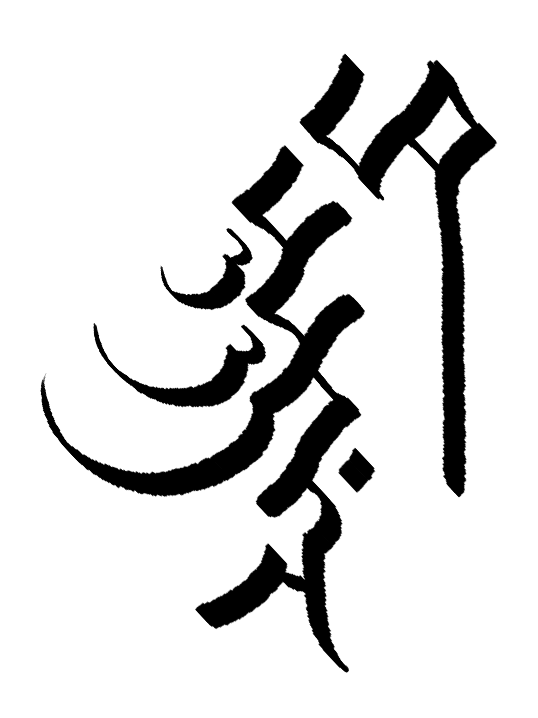
\includegraphics[scale=2.1]{scriptchapter.png}

    \emph{``beauty from discipline.''}
\end{center}

\pagebreak

\section{Functioning of the abugida}

The Flavan script is an abugida: the main series of glyphs (called ``the adults'') represent consonantal sounds, while secondary glyphs (called ``the children'') attached to the adults represent vowels following them.

To be more precise, adults mark consonant \emph{clusters}. When writing a word, the entire group of consonants between one vowel and the next is one cluster and maps to one adult. For example, consider the word \textbf{syrbattam}, \emph{room}; if it were to be written it would be decomposed as such\footnote{\textbf{syrbattam} is actually pronounced \apa{s\s{r}"bat:am} with a syllabic \apa{r}, however for the sake of the Flavan script phonological rules such as the contraction \ipa{1r} \textrightarrow \apa{\s{r}} are ignored.}

\begin{center}
    \Large (s)\textsuperscript{y}(rb)\textsuperscript{a}(tt)\textsuperscript{a}(m)
\end{center}

It would therefore be written as the \textbf{s} adult with the \textbf{y} child attached, the \textbf{rb} adult with the \textbf{a} child attached, and so on.

If the word starts in a vowel, we use a ``carrier'' adult called the \textbf{pode} (\textbf{-}). For example, \textbf{arbyd}, \emph{river} would be

\begin{center}
    \LARGE (-)\textsuperscript{a}(rb)\textsuperscript{y}(d)
\end{center}

Note you cannot ``compose'' the \textbf{r} and \textbf{b} adults to make \textbf{rb}. They are separate phonemes and glyphs in Flavan. The Flavan script can only represent words that follow the phonotactical rules, so only those that alternate vowels with allowed consonant clusters. \textbf{andra} is not a Flavan word and it cannot be written because there is no \textbf{ndr} adult.

Words with consecutive vowels can occasionally appear though. These can easily be written using podes.

\subsection{The letter ``a''}

There is \textbf{no letter a}. By default, unmarked adults carry an \textbf{a} vowel, unless at word end. So really, \textbf{syrbattam} should be

\begin{center}
    \Large (s)\textsuperscript{y}(rb)\textsuperscript{unmarked}(tt)\textsuperscript{unmarked}(m)
\end{center}

But what if a word ends in \textbf{a}? Just add more podes. \textbf{gydda}, \emph{love} is

\begin{center}
    \Large (g)\textsuperscript{y} (dd)\textsuperscript{unmarked}(-)\textsuperscript{unmarked}
\end{center}

To be exact, what's happening here is that the final (-) makes it so (dd) is not final anymore, and thus does carry \textbf{a} being unmarked. The (-) here does not contribute any sound by itself.

\section{Visual guidelines}

\vfill

\begin{minipage}{0.5\textwidth}
Flavan is written top to bottom, right to left. Running through the middle of a single column of text is a (partially imaginary) line, the main stem. The adults are placed one below the other, centered on the stem; the centering is essential for readability. You're always allowed to play around with the distance between stems and also with the height of the beginning of each column of text, for aesthetic purposes; however, the stem should \emph{never} bend or be curved or diagonal (except for some very wild designs), and adults should be correctly centered. 

These are valid stem lines. Spacing and starting height are inconsistent, but all stems are perfectly vertical and straight.
\end{minipage}
\hfill
\begin{minipage}{0.45\textwidth}
    \centering
    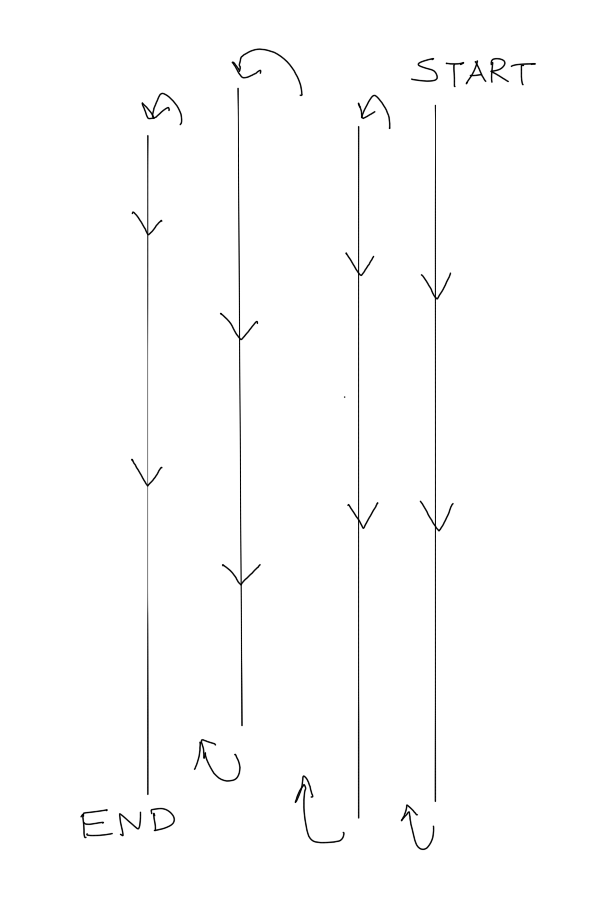
\includegraphics{stems}
\end{minipage}


\vfill

\begin{minipage}{0.45\textwidth}
     \centering
    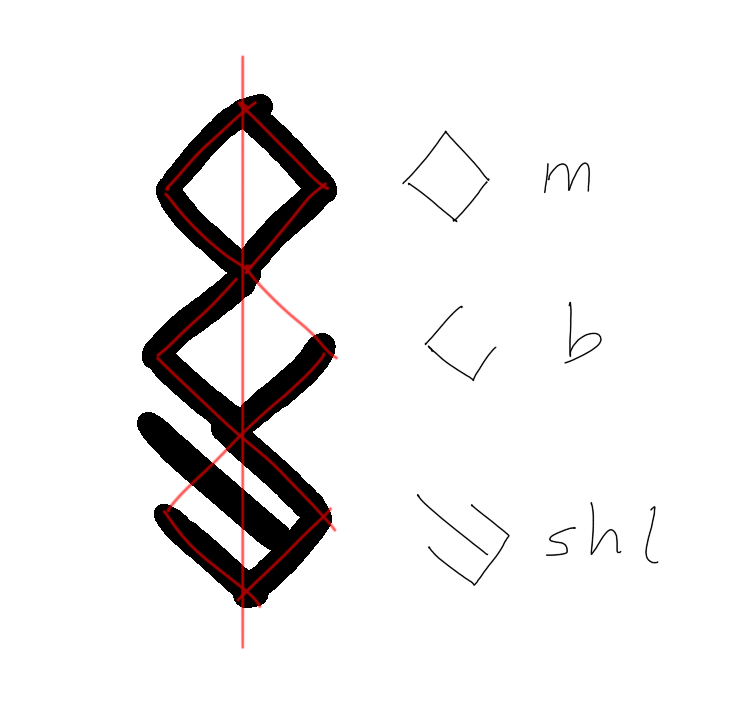
\includegraphics{mabashl}
\end{minipage}
\hfill
\begin{minipage}{0.5\textwidth}
The stem is included literally in some adults, so that words can appear as single connected shapes spanning vertically. Other adults break the stem line, so a disconnected symbol does \textbf{not} mean a word boundary. 

The adults themselves are all built, fundamentally, on a ``template'' of a 45\degree-rotated square, at least in the basic ``geometric'' style. The resulting visual coherence helps in distinguishing glyphs: each square is an adult. For example, the (imaginary) word \textbf{mabashl}, with adults \textbf{m}, \textbf{b}, \textbf{shl} becomes as on the left.

\end{minipage}

\vfill

\begin{minipage}[]{0.5\textwidth}
    Some rules are meant to be broken. Some really aren't. You can for example break free of the grid's vertical constraints. In the right example, the (again imaginary) word \textbf{damard} was stylized by stretching the vertical letter \textbf{d}; this is ok because this glyph, while meant to fit in a template square, does not really follow the lines of the square at all. Moreover, the two lower squares have been stretched into rhombi, and some curvature has been added to the lines. However, both rhombi are equal (approximately) in width and height. In general, stylization (at least for the Demorog script) can result in deformation of the fundamental square shape and stretching of non-square elements, but whenever the deformed squares appear, they should be consistent. This is essential for distinguishing adult boundaries (is there a joke here?).
\end{minipage}
\hfill
\begin{minipage}{0.45\textwidth}
    \centering
    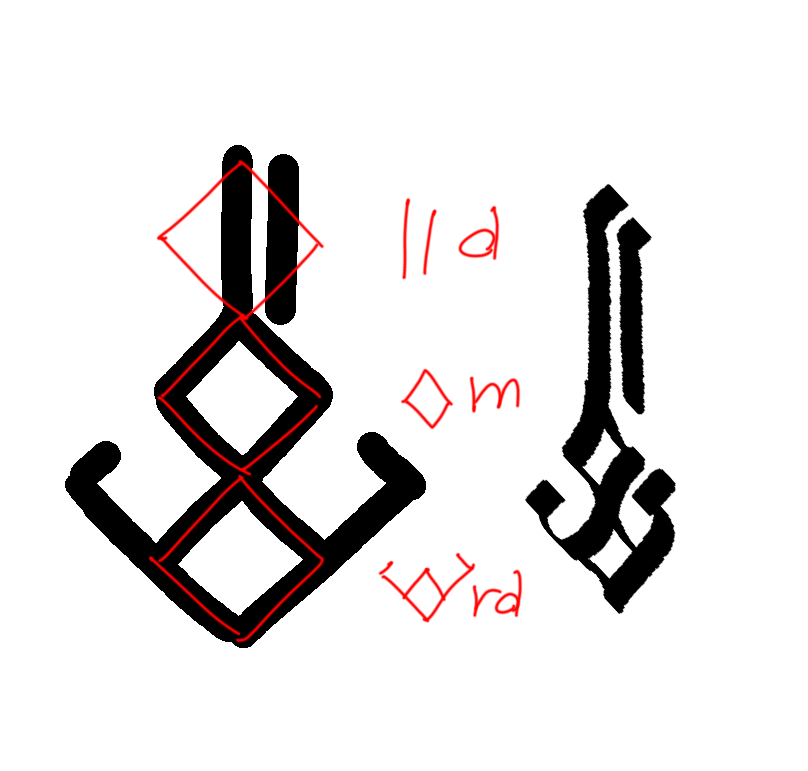
\includegraphics{damard}
\end{minipage}

\vfill

\pagebreak


\section{Children}

\begin{center}
    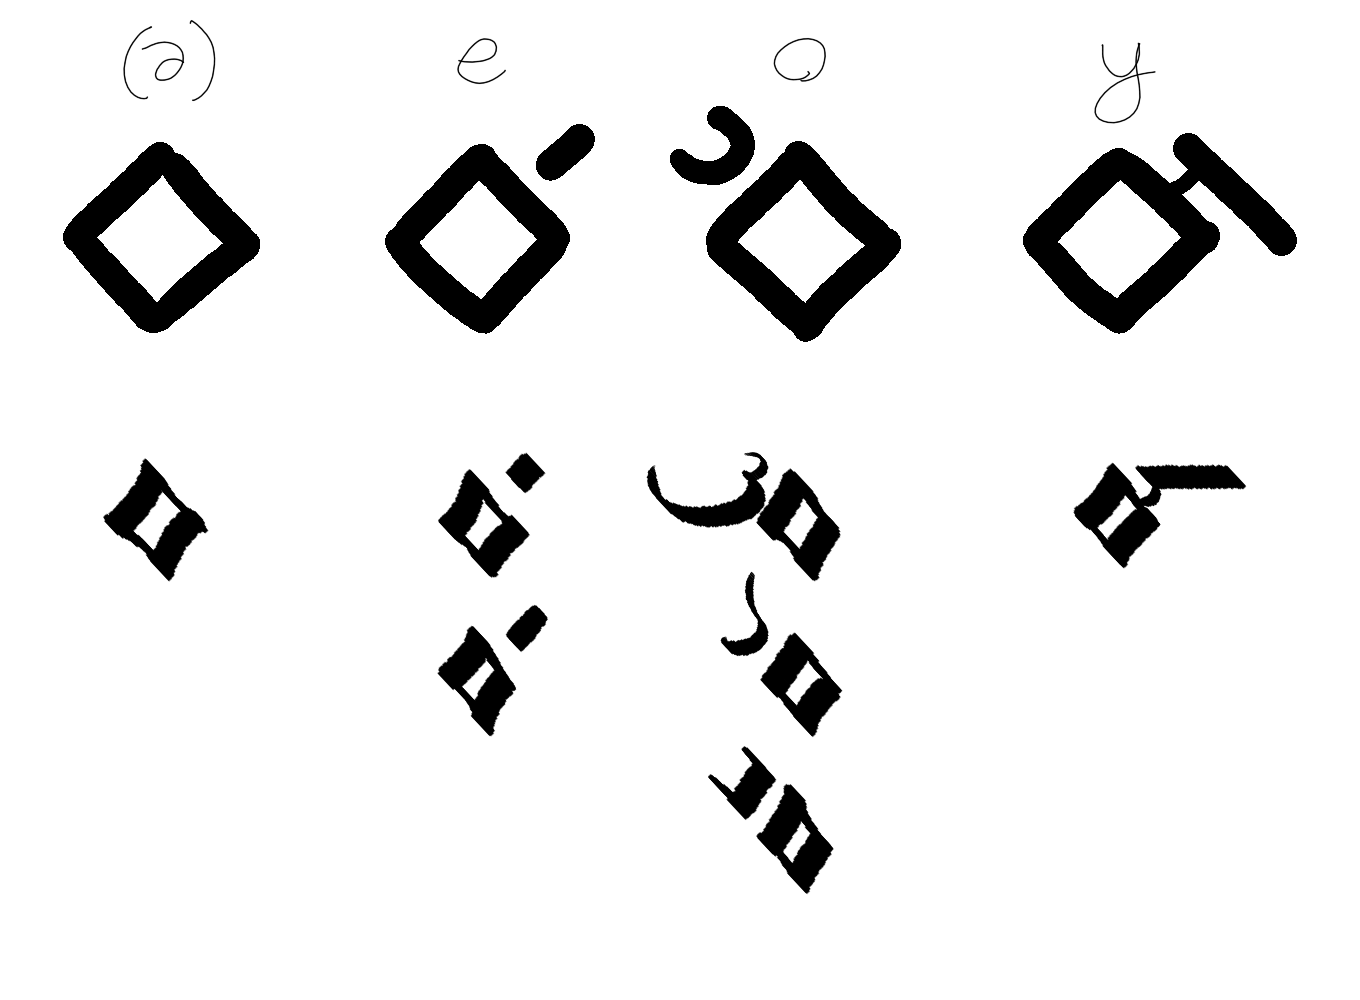
\includegraphics{childrenguide}
\end{center}

The four children markings (the absence of a marking is also considered a vowel letter by Flavans) are depicted here on the letter \textbf{m}. Below, a few variants for the cursive style are presented. There is great freedom in stylization of position and shape of vowel markings, because there is little chance of ambiguity; this freedom should be employed to avoid overlap of the markings with the previous adult. Some guidelines should be however satisfied to guarantee legibility:

\begin{itemize}
    \item \textbf{e} should always be detached from all adults and children on the same column and to the right of its parent adult, \textbf{upper} right if the adult includes a guide square. It should be either dot-like or angle upwards going to the right. It should be straight.
    \item \textbf{o} should also be detached from all glyphs of the column and on the left or upper left of its adult. It can take a great variety of shapes, generally c-like curves with the opening to the upper left, and might include one, two, or even three arcs. On many adults, however, the \textbf{o} and the adult join to create another form (generally it turns into a ``hook'' for the adult), the full syllabary table includes all possible combinations.
    \item \textbf{y} is attached by a little stem to its parent adult. Otherwise, it should not attach to anything else in the same column. The point of attachement is specific to each letter (see the full syllabary table) but it's always either right or upper right. The main stroke angles downward in the strict geometric style but is horizontal in handwritten geometric or in cursive.
\end{itemize}





\section{Syllabary (Males)}
The following are adult-child combination for the ``common'' adults, the ``males'', in geometric style. Some non-obvious cursive version of the geometric glyphs are depicted to their lower-right. The combination \textbf{ngy} contains in the cursive script the only permissible intersection of strokes. Note that the glyphs \textbf{g} and \textbf{s} interrupt the stem above, so there is a space between the adult and the one before. Similarly, \textbf{k} breaks below, and \textbf{t} breaks both above and below.

\begin{center}
    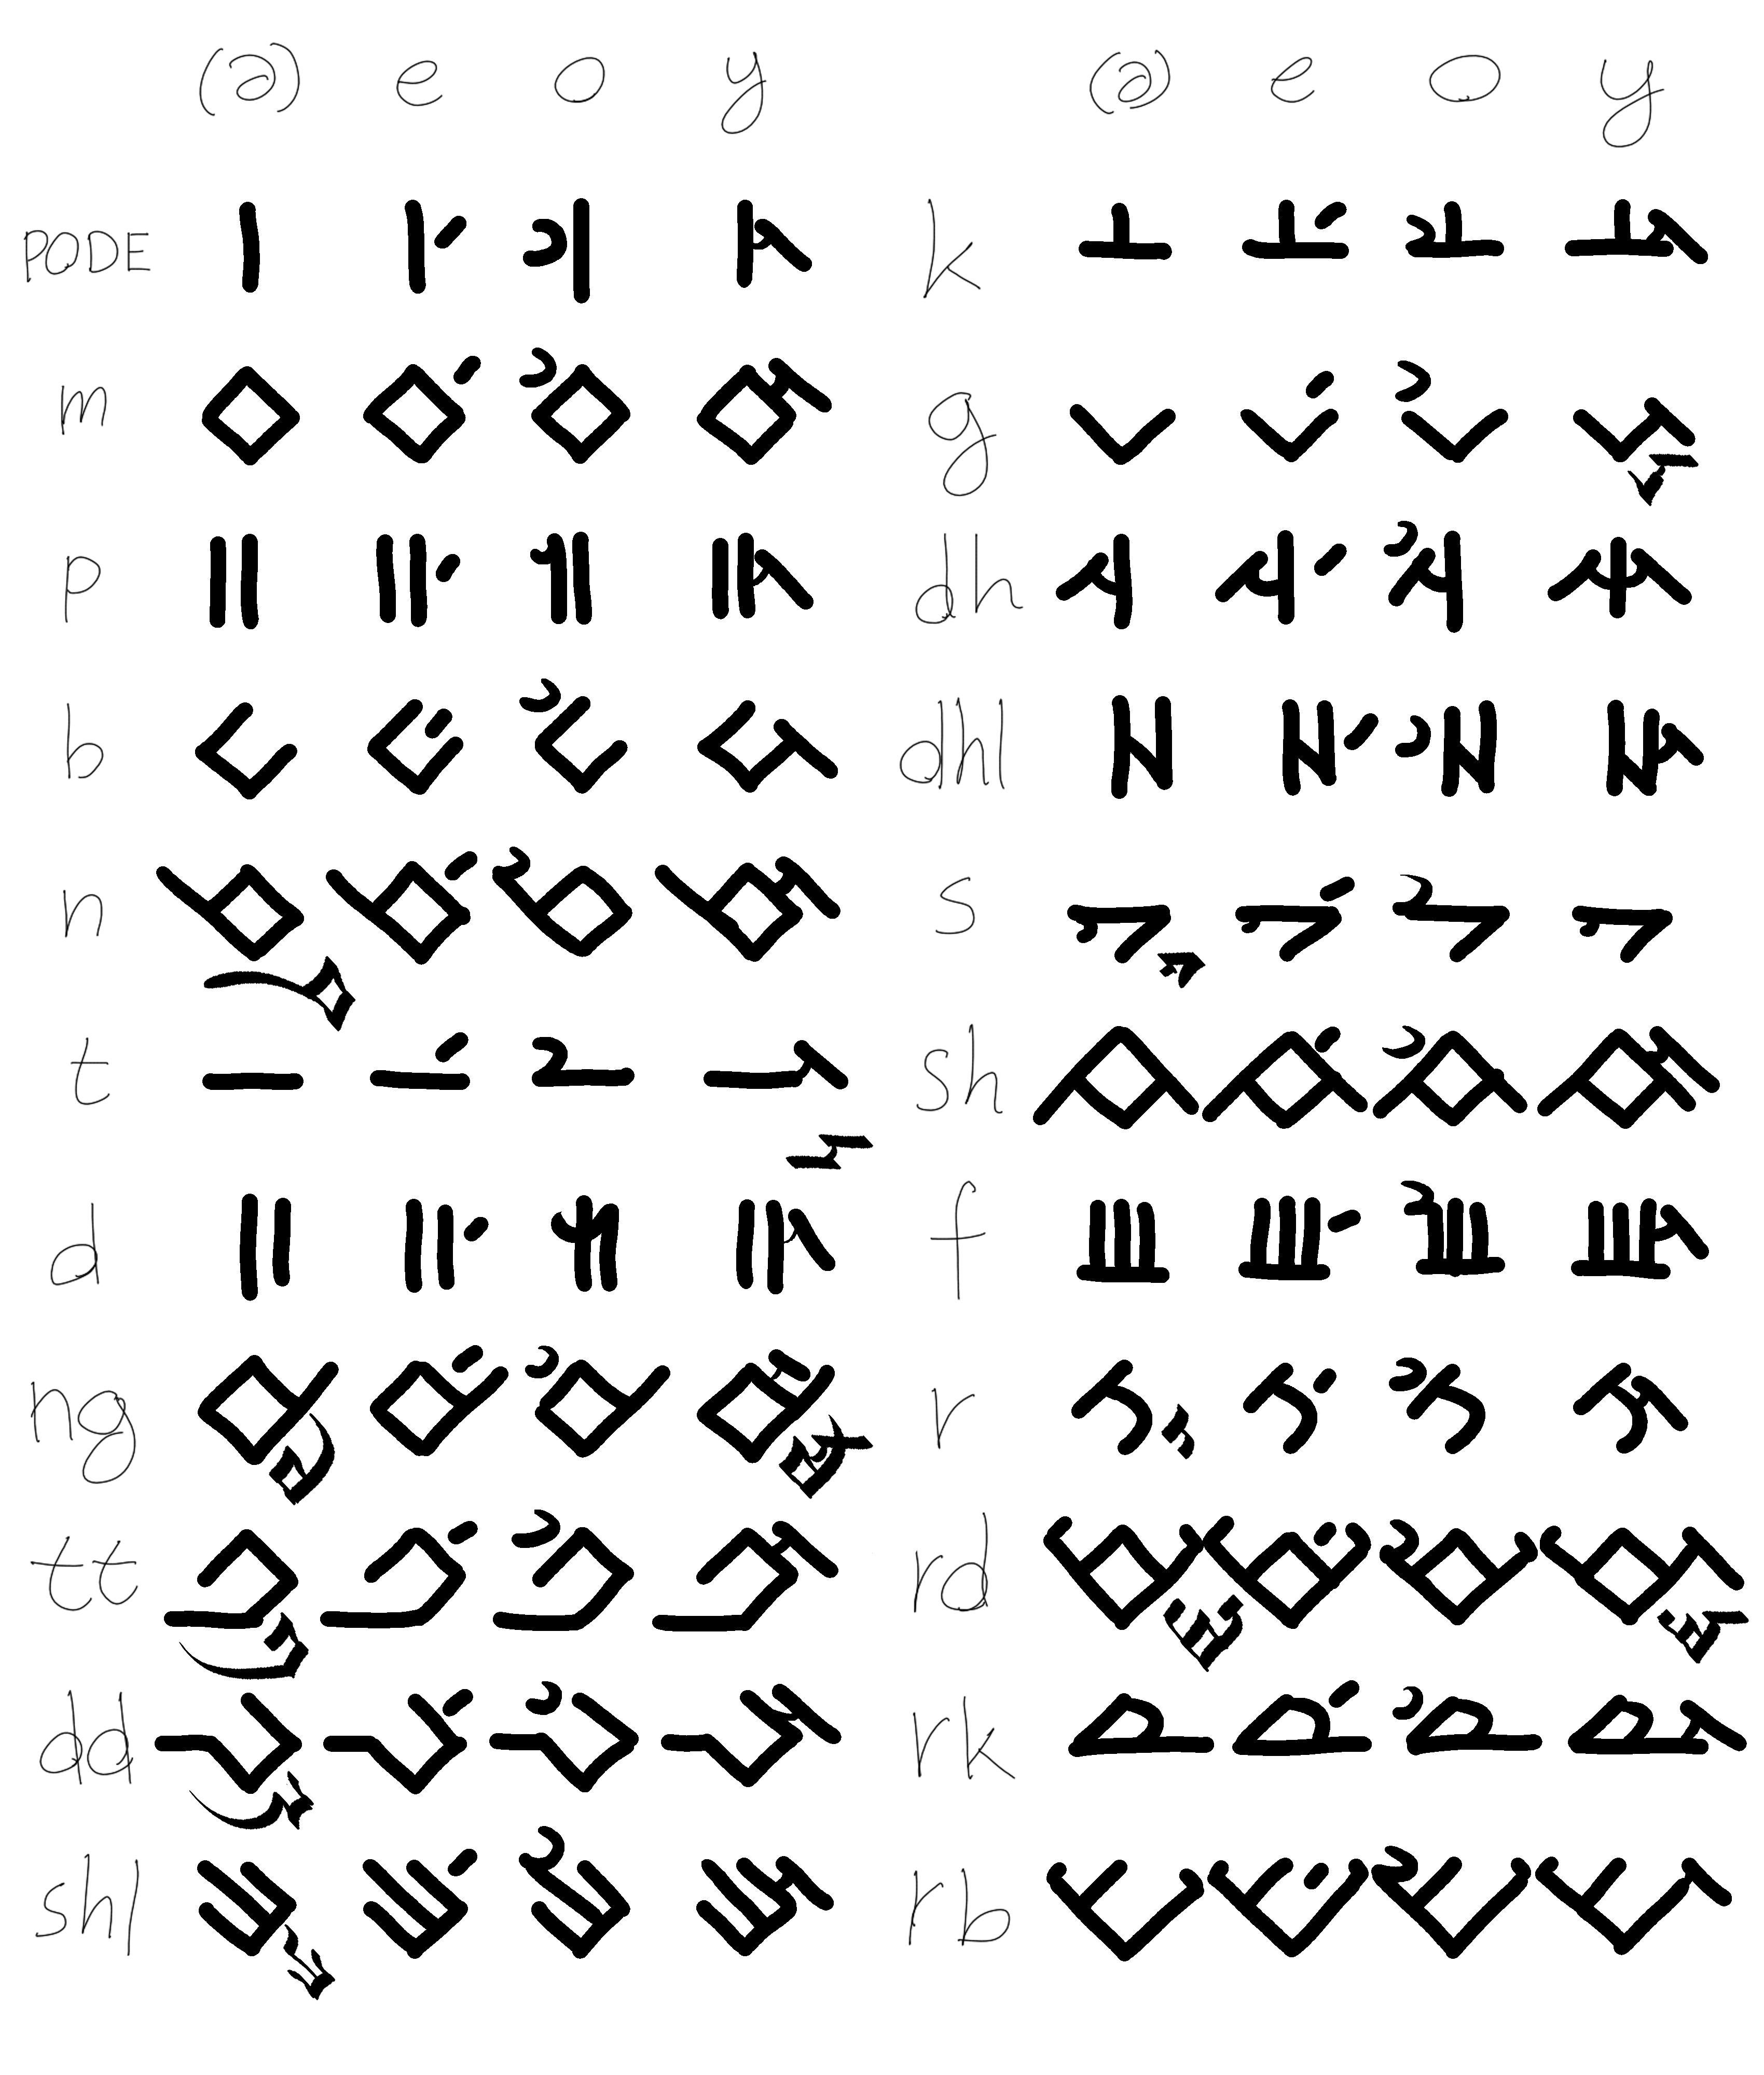
\includegraphics[scale=0.60]{syllabary_males}
\end{center}


%\pagebreak

\begin{samepage}

\section{Syllabary (Females)}
    And here are the more ``uncommon'' glyphs, the ``females''. \textbf{ttk} and \textbf{ttg} are identical; the only distinguishing feature is that the former does not interrupt the main stem while the latter does (and there's a corresponding space before the next letter). The very rare \textbf{pd} glyph must necessarily be drawn bigger than a square in the cursive script for the strokes to be distinct.
\
\begin{center}
    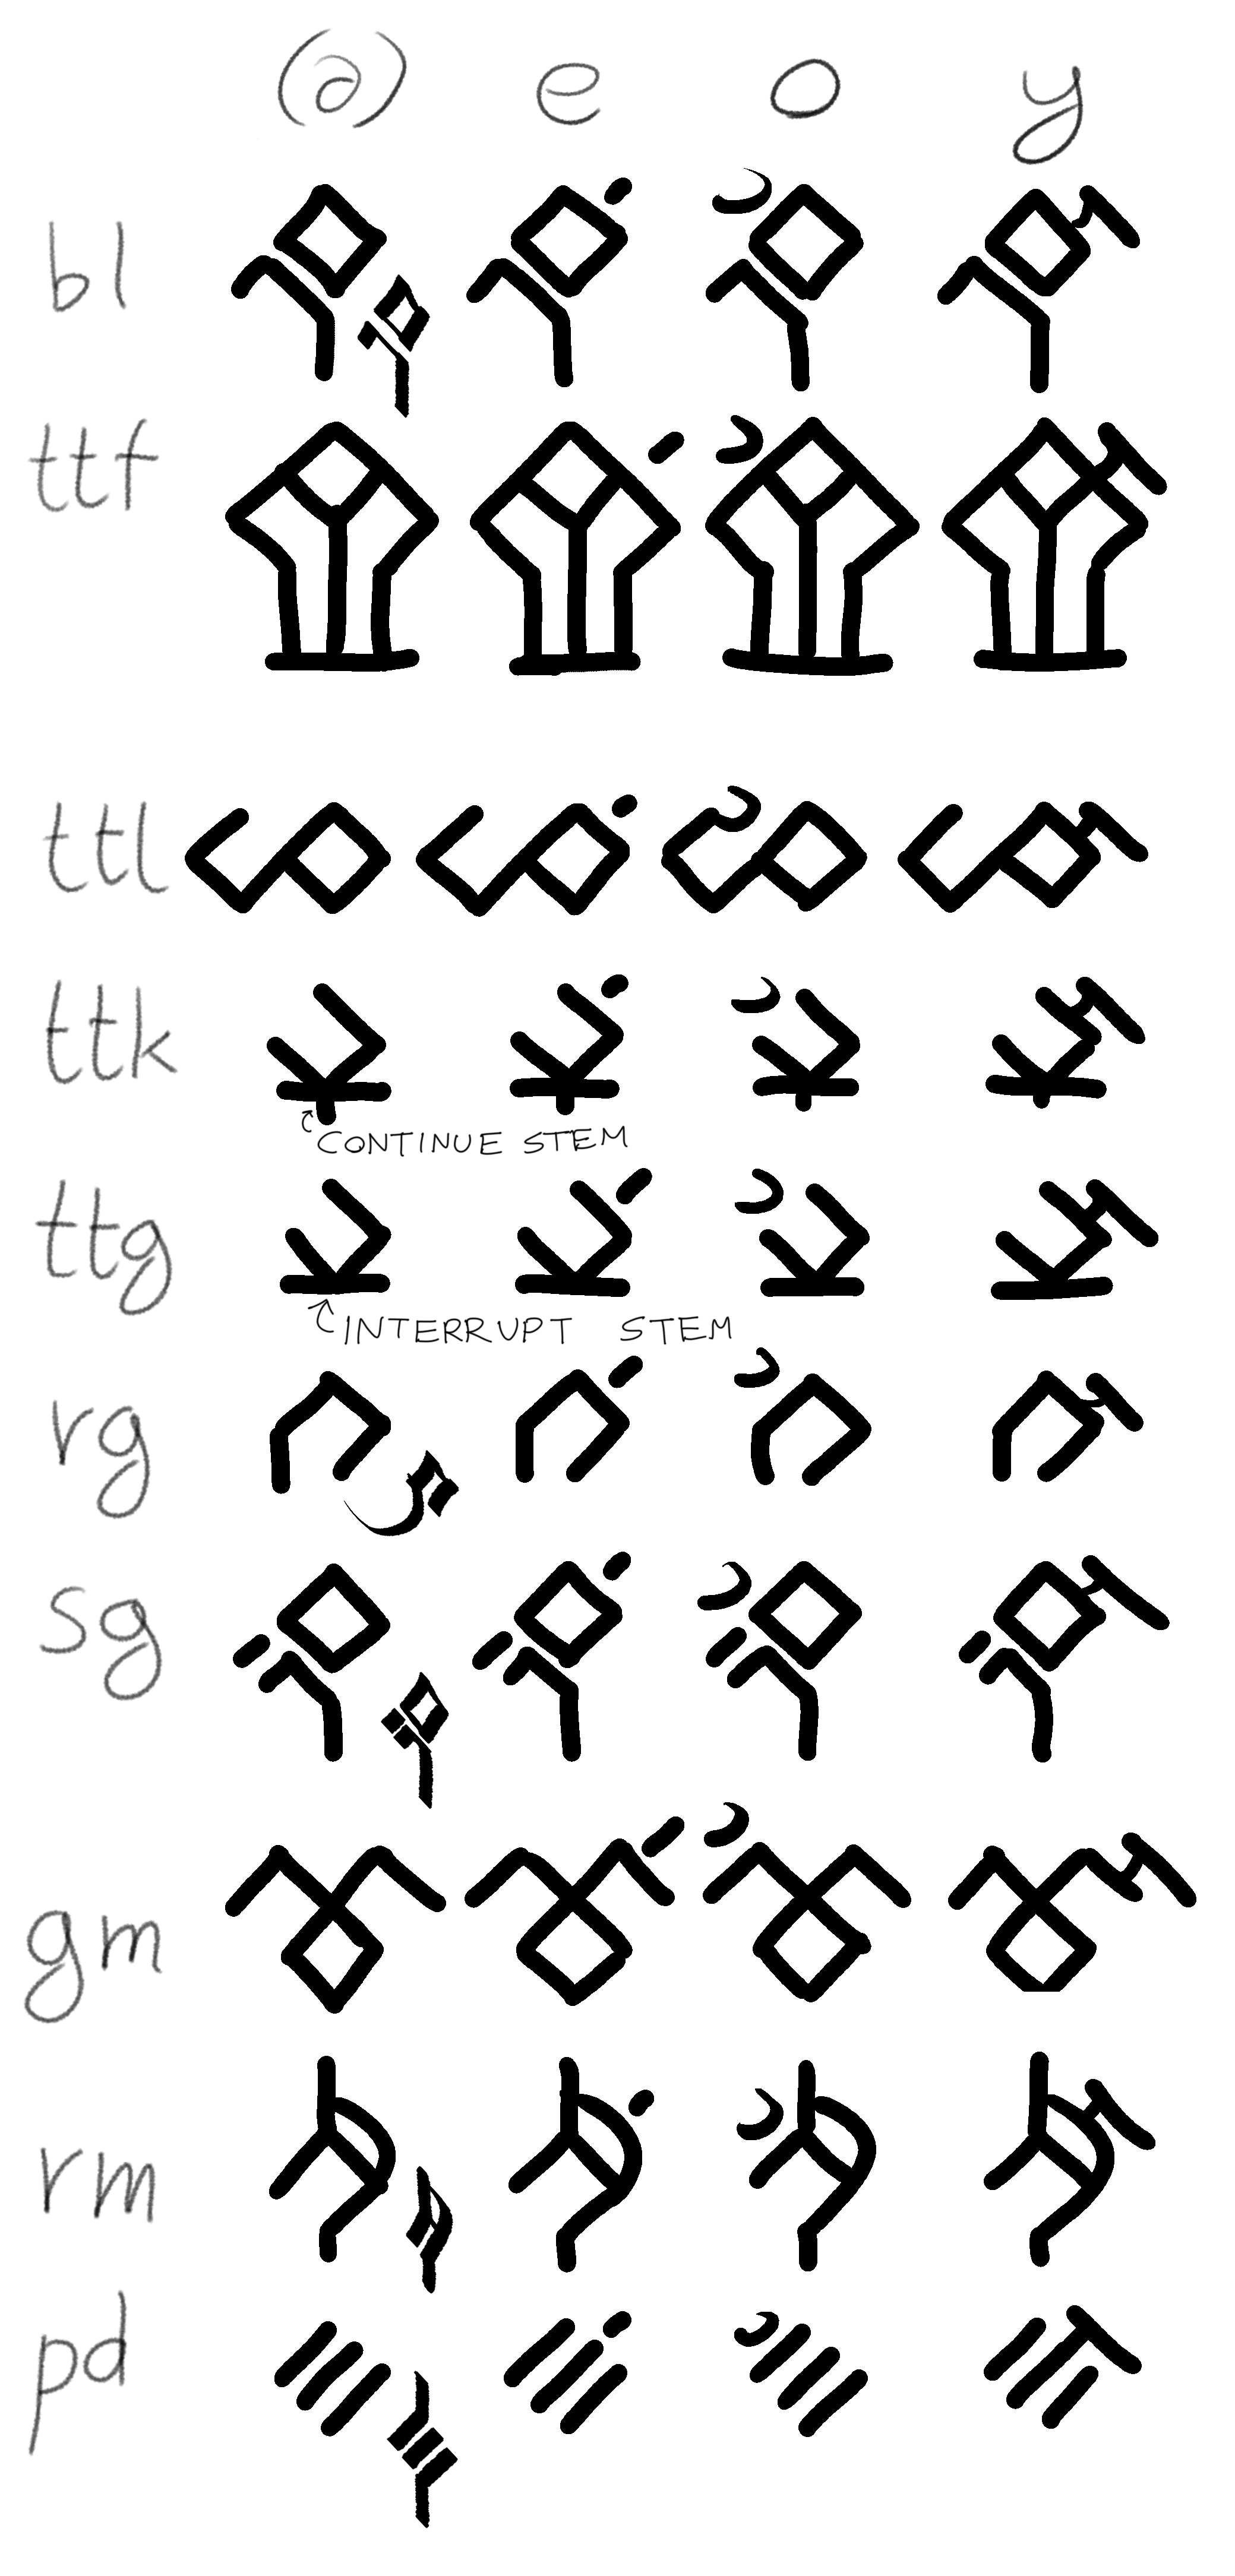
\includegraphics[scale=0.60]{syllabary_females}
\end{center}

\end{samepage}

\pagebreak




\section{Orthography and punctuation}

\vfill

\begin{minipage}[]{0.5\textwidth}
    There's one last ``letter'' to add: by reducing the space between consecutive \textbf{k} and \textbf{t} letters, one obtains a glyph for \textbf{kt}, representing the sound \apa{kt}. This can only be word-final and it's generally a consequence of a genitive ending where the last vowel has disappeared. In the rare case that a word does literally end in \textbf{kat}, an extra amount of space has to be introduced to clarify this.
\end{minipage}
\hfill
\begin{minipage}[]{0.45 \textwidth}
    \centering
    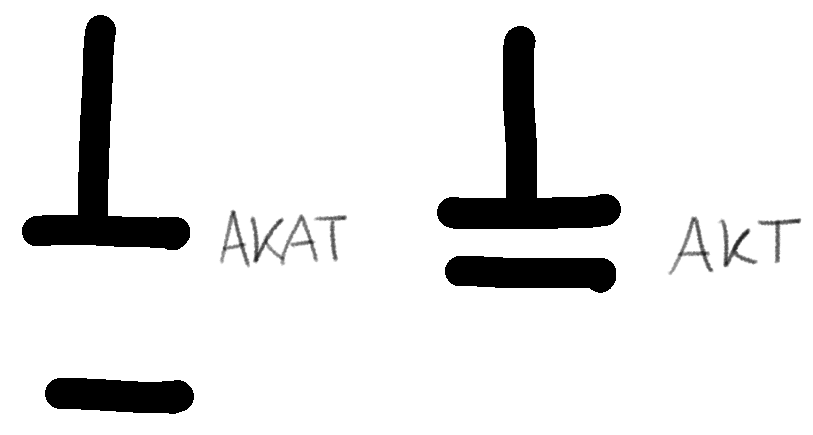
\includegraphics{kt}
\end{minipage}

\vfill

\begin{minipage}[]{0.45\textwidth}
    \centering
    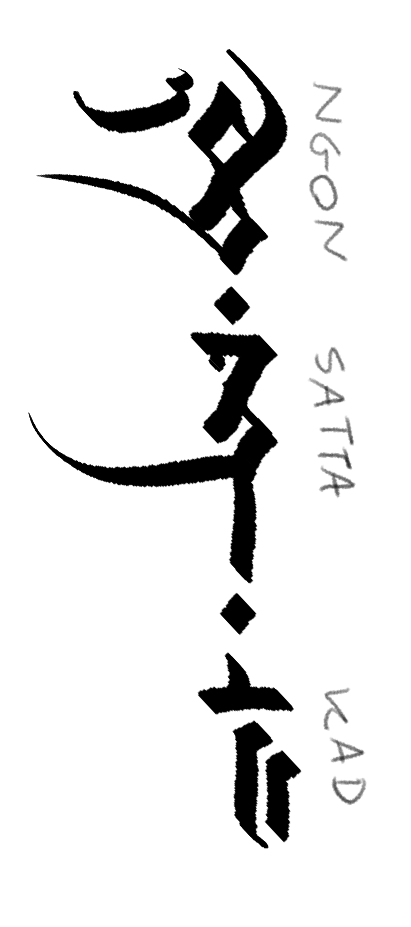
\includegraphics{ngonsettakad}
\end{minipage}
\hfill
\begin{minipage}[]{0.5\textwidth}
    Dots (or small strokes) aligned with the stem line separate words. They are identical to the \textbf{e} marking except for the positioning, in all styles. Words \textbf{never} span multiple columns, and no marking is placed when the column ends.

    Note that Flavans might separate words differently than the standard employed romanization, and that there are numerous irregularities and regional variants to this.
\end{minipage}

\vfill
\vspace{-50pt}

\begin{minipage}[]{0.5\textwidth}
    Three dots in a triangle mark the beginning of a quote, song, or direct speech. Two dots are sometimes (but not often, and surely not consistently) used to separate long periods or sentences. Three dots in text mark that the following is a name (signature, author, reference).
\end{minipage}
\hfill
\begin{minipage}[]{0.45\textwidth}
    \centering
    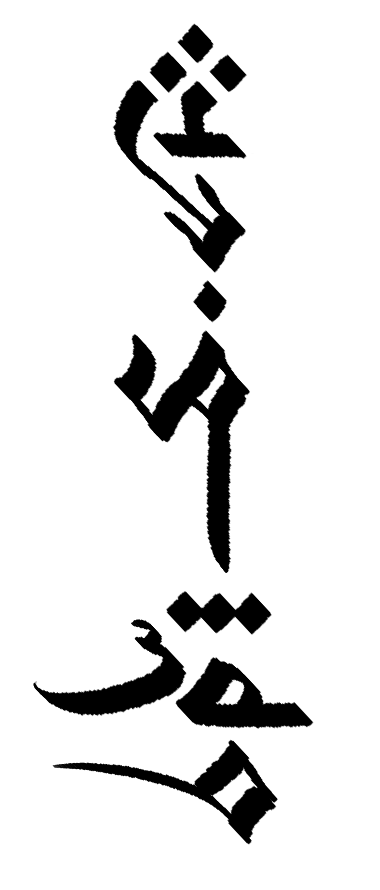
\includegraphics{piss}
\end{minipage}

\vfill


\vspace{-50pt}

\begin{minipage}[]{0.45\textwidth}
    \centering
    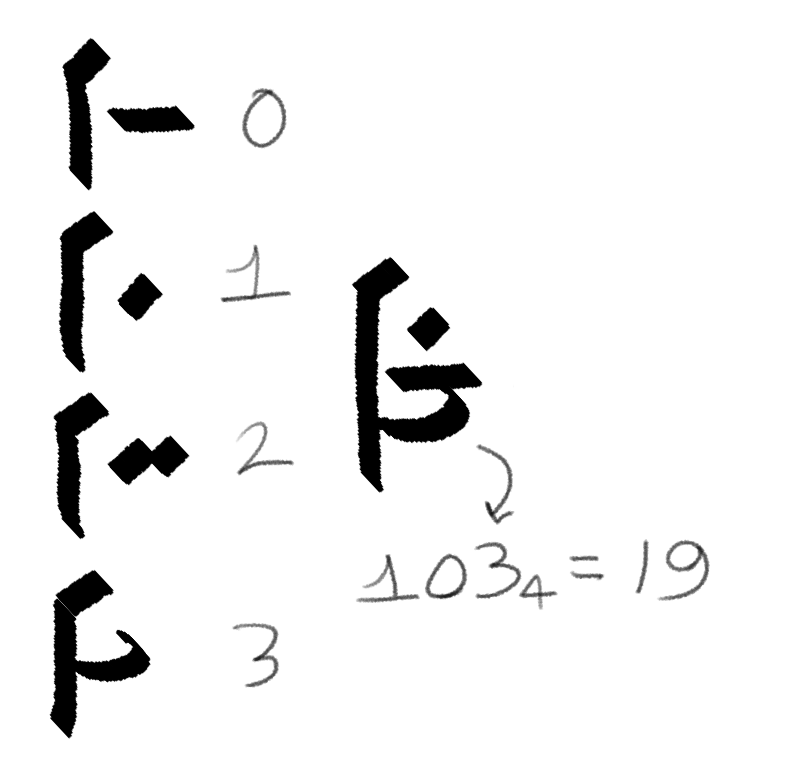
\includegraphics{digits}
\end{minipage}
\hfill
\begin{minipage}[]{0.5\textwidth}
    Flavans, after way more careful deliberation than was honestly necessary, have settled on a positional system for writing numbers, the \textbf{Borg system}. To write a number, draw a pode, then draw its digits in base $4$ from top to bottom using the scheme to the left.
\end{minipage}



\vfill

\end{document}
